% Relatorio da etapa 0 do plano de trabalho (../README.md): fechar o que ja rodava antes das etapas no fermi. Para refazer:
% ./atualiza.sh, que roda
%   python3 -I figuras_etapa0.py   (figuras em figs/fig_e0_*.pdf e numeros_etapa0.tex; imprime cada numero com o arquivo
%                                   de onde sai)
% e compila este arquivo duas vezes numa pasta temporaria. Nenhum numero dos dados esta escrito aqui: todos vem das macros
% do numeros_etapa0.tex.
\documentclass[11pt,a4paper]{article}
\usepackage[T1]{fontenc}\usepackage[utf8]{inputenc}\usepackage[brazilian]{babel}\usepackage{lmodern}
\usepackage[margin=2.2cm]{geometry}\usepackage{booktabs}\usepackage{graphicx}\usepackage{caption}
\usepackage{float}\usepackage[hidelinks]{hyperref}\usepackage{amsmath}\usepackage{amssymb}\usepackage{microtype}
\usepackage{array}
\captionsetup{font=small}
\renewcommand{\topfraction}{0.9}\renewcommand{\bottomfraction}{0.8}\renewcommand{\textfraction}{0.07}
\renewcommand{\floatpagefraction}{0.75}
\graphicspath{{figs/}}
% gerado por figuras_etapa0.py em 15/11/2026 12:16: nao edite (rode o script de novo)
\newif\ifchofim \chofimfalse
\newif\ifpcparou \pcparoutrue
\newif\ifchocincopronto \chocincoprontofalse
\newif\ifchocincopiloto \chocincopilotofalse
\newif\ifchoaicincoiniciado \choaicincoiniciadofalse
\newif\ifchoaicincopronto \choaicincoprontofalse
\newif\ifchoaicincofalhas \choaicincofalhasfalse
\newif\ifchosetepronto \choseteprontofalse
\newif\ifchosetepiloto \chosetepilotofalse
\newif\ifchoaiseteiniciado \choaiseteiniciadofalse
\newif\ifchoaisetepronto \choaiseteprontofalse
\newif\ifchoaisetefalhas \choaisetefalhasfalse
\newif\ifformdezpronto \formdezprontofalse
\newif\ifformdezpassoacima \formdezpassoacimatrue
\newif\ifformvintepronto \formvinteprontofalse
\newif\ifformvintepassoacima \formvintepassoacimatrue
\newif\ifaiforminiciado \aiforminiciadofalse
\newif\ifaiformfalhas \aiformfalhasfalse
\newif\ifaiformpronto \aiformprontofalse
\newif\ifchoburaco \choburacotrue
\newcommand{\HoraDados}{15/11/2026, 12h16} % relogio do PC ao rodar o script
\newcommand{\MinWilson}{20} % ../README.md (criterios gerais)
\newcommand{\RbNDireto}{2000} % numeros_rebaixamento.tex (relatorio_rebaixamento.pdf)
\newcommand{\RbNfDireto}{314} % numeros_rebaixamento.tex (relatorio_rebaixamento.pdf)
\newcommand{\RbPfDireto}{15{,}70} % numeros_rebaixamento.tex (relatorio_rebaixamento.pdf)
\newcommand{\RbCovPfDireto}{5{,}2} % numeros_rebaixamento.tex (relatorio_rebaixamento.pdf)
\newcommand{\RbNBanda}{1000} % numeros_rebaixamento.tex (relatorio_rebaixamento.pdf)
\newcommand{\RbPfBanda}{15{,}87} % numeros_rebaixamento.tex (relatorio_rebaixamento.pdf)
\newcommand{\RbCovPfBanda}{4{,}4} % numeros_rebaixamento.tex (relatorio_rebaixamento.pdf)
\newcommand{\RbDifBanda}{0{,}16} % numeros_rebaixamento.tex (relatorio_rebaixamento.pdf)
\newcommand{\RbGanhoBanda}{2{,}7} % numeros_rebaixamento.tex (relatorio_rebaixamento.pdf)
\newcommand{\RbGanhoLinear}{4{,}0} % numeros_rebaixamento.tex (relatorio_rebaixamento.pdf)
\newcommand{\RbFracGanhoBanda}{69} % numeros_rebaixamento.tex (relatorio_rebaixamento.pdf)
\newcommand{\RbMuDoisBanda}{2{,}06} % numeros_rebaixamento.tex (relatorio_rebaixamento.pdf)
\newcommand{\RbSC}{\ensuremath{-}1{,}30} % numeros_rebaixamento.tex (relatorio_rebaixamento.pdf)
\newcommand{\RbSPhi}{\ensuremath{-}0{,}49} % numeros_rebaixamento.tex (relatorio_rebaixamento.pdf)
\newcommand{\RbSK}{\ensuremath{-}0{,}36} % numeros_rebaixamento.tex (relatorio_rebaixamento.pdf)
\newcommand{\RbKModos}{20} % numeros_rebaixamento.tex (relatorio_rebaixamento.pdf)
\newcommand{\RbNModos}{1000} % numeros_rebaixamento.tex (relatorio_rebaixamento.pdf)
\newcommand{\RbPfModos}{17{,}89} % numeros_rebaixamento.tex (relatorio_rebaixamento.pdf)
\newcommand{\RbCovPfModos}{6{,}2} % numeros_rebaixamento.tex (relatorio_rebaixamento.pdf)
\newcommand{\RbDifModos}{1{,}58} % numeros_rebaixamento.tex (relatorio_rebaixamento.pdf)
\newcommand{\RbGanhoModos}{1{,}2} % numeros_rebaixamento.tex (relatorio_rebaixamento.pdf)
\newcommand{\RbKNPar}{2000} % numeros_rebaixamento.tex (relatorio_rebaixamento.pdf)
\newcommand{\RbKPfFixo}{13{,}80} % numeros_rebaixamento.tex (relatorio_rebaixamento.pdf)
\newcommand{\RbKPfAleat}{15{,}70} % numeros_rebaixamento.tex (relatorio_rebaixamento.pdf)
\newcommand{\RbKMcNemar}{= 0{,}002} % numeros_rebaixamento.tex (relatorio_rebaixamento.pdf)
\newcommand{\SoBuracoAbaixo}{0} % numeros_solos.tex (relatorio_solos.pdf)
\newcommand{\SoBuracoAcima}{15} % numeros_solos.tex (relatorio_solos.pdf)
\newcommand{\SoBuracoFaixaAbaixo}{$[0{,}9975;\, 1)$} % numeros_solos.tex (relatorio_solos.pdf)
\newcommand{\SoBuracoFaixaAcima}{$[1;\, 1{,}0025)$} % numeros_solos.tex (relatorio_solos.pdf)
\newcommand{\SoBuracoPontos}{1{,}0} % numeros_solos.tex (relatorio_solos.pdf)
\newcommand{\SoBuracoFalta}{10} % numeros_solos.tex (relatorio_solos.pdf)
\newcommand{\SoNCinquenta}{1000} % numeros_solos.tex (relatorio_solos.pdf)
\newcommand{\ChSolo}{f50} % chuva_ai/ref48_piloto/mc_parametros.txt
\newcommand{\ChI}{31{,}05} % chuva_ai/ref48_piloto/mc_parametros.txt
\newcommand{\ChChuva}{24} % chuva_ai/ref48_piloto/mc_parametros.txt
\newcommand{\ChHw}{5} % chuva_ai/ref48_piloto/mc_parametros.txt
\newcommand{\ChTempoPasso}{6} % chuva_ai/ref48_piloto/mc_parametros.txt
\newcommand{\ChTempoFim}{48} % chuva_ai/ref48_piloto/mc_parametros.txt
\newcommand{\ChNTempos}{8} % chuva_ai/ref48_piloto/mc_parametros.txt
\newcommand{\ChCovC}{0{,}3} % chuva_ai/ref48_piloto/mc_parametros.txt
\newcommand{\ChCovPhi}{0{,}1} % chuva_ai/ref48_piloto/mc_parametros.txt
\newcommand{\ChCovK}{0{,}6} % chuva_ai/ref48_piloto/mc_parametros.txt
\newcommand{\ChLx}{20} % chuva_ai/ref48_piloto/mc_parametros.txt
\newcommand{\ChLy}{2} % chuva_ai/ref48_piloto/mc_parametros.txt
\newcommand{\ChKLM}{2000} % chuva_ai/ref48_piloto/mc_parametros.txt
\newcommand{\ChKLvar}{96{,}4} % chuva_ai/ref48_piloto/mc_parametros.txt
\newcommand{\ChMalhaT}{tri2} % chuva_ai/ref48_piloto/mc_parametros.txt
\newcommand{\ChMalhaF}{tri1} % chuva_ai/ref48_piloto/mc_parametros.txt
\newcommand{\ChNref}{4} % chuva_ai/ref48_piloto/mc_parametros.txt
\newcommand{\ChUt}{2} % chuva_ai/ref48_piloto/mc_parametros.txt
\newcommand{\ChSementeP}{2025} % chuva_ai/ref48_piloto/mc_parametros.txt
\newcommand{\ChSementeA}{1} % chuva_ai/ref48_ai/mc_parametros.txt
\newcommand{\ChBandaT}{24} % chuva_ai/ref48_ai/mc_parametros.txt
\newcommand{\ChEliteFrac}{10} % chuva_ai/ref48_ai/mc_parametros.txt
\newcommand{\ChNAlvoP}{200} % cluster/casos_chuva_ai.txt
\newcommand{\ChNAlvoA}{200} % cluster/casos_chuva_ai.txt
\newcommand{\ChDetMin}{1{,}1251} % chuva_ai/ref48_piloto/mc_0_0.csv (realizacao -1)
\newcommand{\ChDetT}{24} % chuva_ai/ref48_piloto/mc_0_0.csv (realizacao -1)
\newcommand{\ChForaP}{0} % chuva_ai/ref48_piloto/mc_*.csv (sem fator ou sem algum instante)
\newcommand{\ChForaA}{0} % chuva_ai/ref48_ai/mc_*.csv (sem fator ou sem algum instante)
\newcommand{\ChPIC}{exato} % IC do piloto (13 falhas)
\newcommand{\ChNP}{200} % chuva_ai/ref48_piloto/mc_*.csv
\newcommand{\ChPNf}{13} % chuva_ai/ref48_piloto/mc_*.csv (FS < 1 em algum instante)
\newcommand{\ChPPf}{6{,}50} % chuva_ai/ref48_piloto/mc_*.csv
\newcommand{\ChPLo}{3{,}5} % chuva_ai/ref48_piloto/mc_*.csv (IC exato)
\newcommand{\ChPHi}{10{,}9} % chuva_ai/ref48_piloto/mc_*.csv (IC exato)
\newcommand{\ChPCov}{26{,}9} % chuva_ai/ref48_piloto/mc_*.csv (s_q / (raiz(N) P_f))
\newcommand{\ChMinNoDet}{199} % chuva_ai/ref48_piloto/mc_*.csv (realizacoes com o minimo no instante do deterministico)
\newcommand{\ChFalhaFora}{0} % chuva_ai/ref48_piloto/mc_*.csv e chuva_ai/ref48_ai/mc_*.csv (FS < 1 noutro instante e >= 1 em 24 h)
\newcommand{\ChFalhaForaFrase}{nenhuma realização das duas amostras falha} % chuva_ai/ref48_piloto/mc_*.csv e chuva_ai/ref48_ai/mc_*.csv
\newcommand{\ChNA}{200} % chuva_ai/ref48_ai/mc_*.csv
\newcommand{\ChANf}{77} % chuva_ai/ref48_ai/mc_*.csv (falhas sorteadas)
\newcommand{\ChAFrac}{38} % chuva_ai/ref48_ai/mc_*.csv
\newcommand{\ChAPf}{6{,}22} % chuva_ai/ref48_ai/mc_*.csv (soma(w I) / N)
\newcommand{\ChAPfArred}{6} % chuva_ai/ref48_ai/mc_*.csv (arredondada)
\newcommand{\ChACov}{13{,}6} % chuva_ai/ref48_ai/mc_*.csv (s_q / (raiz(N) P_f))
\newcommand{\ChALo}{4{,}6} % chuva_ai/ref48_ai/mc_*.csv (P_f (1 - 1,96 CoV))
\newcommand{\ChAHi}{7{,}9} % chuva_ai/ref48_ai/mc_*.csv (P_f (1 + 1,96 CoV))
\newcommand{\ChAPesoMedio}{0{,}939} % chuva_ai/ref48_ai/mc_*.csv
\newcommand{\ChAPesoSe}{0{,}117} % chuva_ai/ref48_ai/mc_*.csv (desvio da media)
\newcommand{\ChAPesoCompat}{compatível com 1} % chuva_ai/ref48_ai/mc_*.csv (|media - 1| / desvio = 0.52)
\newcommand{\ChAEss}{49} % chuva_ai/ref48_ai/mc_*.csv ((soma w)^2 / soma w^2)
\newcommand{\ChAEssF}{43} % chuva_ai/ref48_ai/mc_*.csv (ESS das falhas: (soma q)^2 / soma q^2)
\newcommand{\ChPEssF}{13} % chuva_ai/ref48_piloto/mc_*.csv (ESS das falhas: no direto, n_f)
\newcommand{\ChPParcela}{8} % chuva_ai/ref48_piloto/mc_*.csv (maior parcela: no direto, 1 / n_f)
\newcommand{\AlertaParcela}{10} % ../README.md (criterios gerais)
\newcommand{\ChAPesoFalha}{0{,}16} % chuva_ai/ref48_ai/mc_*.csv (peso medio nas falhas)
\newcommand{\ChAPesoFalhaMax}{0{,}67} % chuva_ai/ref48_ai/mc_*.csv (maior peso nas falhas)
\newcommand{\ChAPesoMax}{9{,}8} % chuva_ai/ref48_ai/mc_*.csv (maior peso)
\newcommand{\ChAParcela}{5} % chuva_ai/ref48_ai/mc_*.csv (maior w I / soma w I)
\newcommand{\ChDif}{\ensuremath{-}0{,}14} % chuva_ai/ref48_ai/mc_*.csv e chuva_ai/ref48_piloto/mc_*.csv (desvios)
\newcommand{\ChDifPontos}{\ensuremath{-}0{,}28} % chuva_ai/ref48_ai/mc_*.csv e chuva_ai/ref48_piloto/mc_*.csv
\newcommand{\ChGanho}{4{,}1} % chuva_ai/ref48_ai/mc_*.csv ((CoV do direto com N e P_f da AI / CoV da AI)^2)
\newcommand{\ChRazao}{0{,}24} % chuva_ai/ref48_ai/mc_*.csv (1 / ganho)
\newcommand{\ChCovMesmoN}{27{,}5} % raiz((1 - P_f) / (N P_f)) com N e P_f da AI
\newcommand{\ChNParaCov}{820} % (1 - P_f) / (P_f CoV^2) com os da AI
\newcommand{\ChVies}{sem sinal de viés} % chuva_ai/ref48_ai/mc_*.csv
\newcommand{\ChTSeis}{6} % chuva_ai/ref48_piloto/mc_parametros.txt (TEMPOS)
\newcommand{\ChPfASeis}{0{,}00} % chuva_ai/ref48_ai/mc_*.csv (P_f em 6 h)
\newcommand{\ChCovASeis}{--} % chuva_ai/ref48_ai/mc_*.csv (CoV em 6 h)
\newcommand{\ChNfPSeis}{0} % chuva_ai/ref48_piloto/mc_*.csv (FS < 1 em 6 h)
\newcommand{\ChFalhasPSeis}{nenhuma falha} % chuva_ai/ref48_piloto/mc_*.csv (FS < 1 em 6 h)
\newcommand{\ChTDoze}{12} % chuva_ai/ref48_piloto/mc_parametros.txt (TEMPOS)
\newcommand{\ChPfADoze}{0{,}00} % chuva_ai/ref48_ai/mc_*.csv (P_f em 12 h)
\newcommand{\ChCovADoze}{--} % chuva_ai/ref48_ai/mc_*.csv (CoV em 12 h)
\newcommand{\ChNfPDoze}{0} % chuva_ai/ref48_piloto/mc_*.csv (FS < 1 em 12 h)
\newcommand{\ChFalhasPDoze}{nenhuma falha} % chuva_ai/ref48_piloto/mc_*.csv (FS < 1 em 12 h)
\newcommand{\ChTDezoito}{18} % chuva_ai/ref48_piloto/mc_parametros.txt (TEMPOS)
\newcommand{\ChPfADezoito}{0{,}014} % chuva_ai/ref48_ai/mc_*.csv (P_f em 18 h)
\newcommand{\ChCovADezoito}{61} % chuva_ai/ref48_ai/mc_*.csv (CoV em 18 h)
\newcommand{\ChNfPDezoito}{0} % chuva_ai/ref48_piloto/mc_*.csv (FS < 1 em 18 h)
\newcommand{\ChFalhasPDezoito}{nenhuma falha} % chuva_ai/ref48_piloto/mc_*.csv (FS < 1 em 18 h)
\newcommand{\ChTVinteQuatro}{24} % chuva_ai/ref48_piloto/mc_parametros.txt (TEMPOS)
\newcommand{\ChPfAVinteQuatro}{6{,}22} % chuva_ai/ref48_ai/mc_*.csv (P_f em 24 h)
\newcommand{\ChCovAVinteQuatro}{14} % chuva_ai/ref48_ai/mc_*.csv (CoV em 24 h)
\newcommand{\ChNfPVinteQuatro}{13} % chuva_ai/ref48_piloto/mc_*.csv (FS < 1 em 24 h)
\newcommand{\ChFalhasPVinteQuatro}{13 falhas} % chuva_ai/ref48_piloto/mc_*.csv (FS < 1 em 24 h)
\newcommand{\ChTTrinta}{30} % chuva_ai/ref48_piloto/mc_parametros.txt (TEMPOS)
\newcommand{\ChPfATrinta}{0{,}37} % chuva_ai/ref48_ai/mc_*.csv (P_f em 30 h)
\newcommand{\ChCovATrinta}{31} % chuva_ai/ref48_ai/mc_*.csv (CoV em 30 h)
\newcommand{\ChNfPTrinta}{1} % chuva_ai/ref48_piloto/mc_*.csv (FS < 1 em 30 h)
\newcommand{\ChFalhasPTrinta}{1 falha} % chuva_ai/ref48_piloto/mc_*.csv (FS < 1 em 30 h)
\newcommand{\ChTTrintaSeis}{36} % chuva_ai/ref48_piloto/mc_parametros.txt (TEMPOS)
\newcommand{\ChPfATrintaSeis}{0{,}035} % chuva_ai/ref48_ai/mc_*.csv (P_f em 36 h)
\newcommand{\ChCovATrintaSeis}{64} % chuva_ai/ref48_ai/mc_*.csv (CoV em 36 h)
\newcommand{\ChNfPTrintaSeis}{0} % chuva_ai/ref48_piloto/mc_*.csv (FS < 1 em 36 h)
\newcommand{\ChFalhasPTrintaSeis}{nenhuma falha} % chuva_ai/ref48_piloto/mc_*.csv (FS < 1 em 36 h)
\newcommand{\ChTQuarentaDois}{42} % chuva_ai/ref48_piloto/mc_parametros.txt (TEMPOS)
\newcommand{\ChPfAQuarentaDois}{0{,}011} % chuva_ai/ref48_ai/mc_*.csv (P_f em 42 h)
\newcommand{\ChCovAQuarentaDois}{73} % chuva_ai/ref48_ai/mc_*.csv (CoV em 42 h)
\newcommand{\ChNfPQuarentaDois}{0} % chuva_ai/ref48_piloto/mc_*.csv (FS < 1 em 42 h)
\newcommand{\ChFalhasPQuarentaDois}{nenhuma falha} % chuva_ai/ref48_piloto/mc_*.csv (FS < 1 em 42 h)
\newcommand{\ChTQuarentaOito}{48} % chuva_ai/ref48_piloto/mc_parametros.txt (TEMPOS)
\newcommand{\ChPfAQuarentaOito}{0{,}004} % chuva_ai/ref48_ai/mc_*.csv (P_f em 48 h)
\newcommand{\ChCovAQuarentaOito}{100} % chuva_ai/ref48_ai/mc_*.csv (CoV em 48 h)
\newcommand{\ChNfPQuarentaOito}{0} % chuva_ai/ref48_piloto/mc_*.csv (FS < 1 em 48 h)
\newcommand{\ChFalhasPQuarentaOito}{nenhuma falha} % chuva_ai/ref48_piloto/mc_*.csv (FS < 1 em 48 h)
\newcommand{\ChLinhasInstantes}{6 & 1{,}7777 & 1{,}7670 & 6{,}1 & 0 & 0 & 0 & -- \\
  12 & 1{,}4983 & 1{,}4788 & 6{,}7 & 0 & 0 & 0 & -- \\
  18 & 1{,}2751 & 1{,}2664 & 7{,}1 & 0 & 0 & 0{,}014 & 61 \\
  24 & 1{,}1251 & 1{,}1297 & 7{,}7 & 13 & 6{,}50 & 6{,}22 & 14 \\
  30 & 1{,}1973 & 1{,}1979 & 7{,}0 & 1 & 0{,}50 & 0{,}37 & 31 \\
  36 & 1{,}2501 & 1{,}2447 & 6{,}9 & 0 & 0 & 0{,}035 & 64 \\
  42 & 1{,}2894 & 1{,}2824 & 6{,}8 & 0 & 0 & 0{,}011 & 73 \\
  48 & 1{,}3225 & 1{,}3162 & 6{,}7 & 0 & 0 & 0{,}004 & 100 \\} % chuva_ai/ref48_piloto/mc_*.csv, chuva_ai/ref48_ai/mc_*.csv (por instante)
\newcommand{\ChZerosA}{6 e 12} % chuva_ai/ref48_ai/mc_*.csv (instantes sem falha sorteada)
\newcommand{\ChZeroHi}{1{,}8} % IC exato com 0 falhas em 200
\newcommand{\ChDeslocBlocos}{200} % chuva_ai/ref48_ai/mc_desloc_*.txt
\newcommand{\ChDeslocIguais}{o mesmo} % chuva_ai/ref48_ai/mc_desloc_*.txt
\newcommand{\ChElite}{20} % chuva_ai/ref48_ai/mc_desloc_*.txt
\newcommand{\ChNivel}{1{,}0079} % chuva_ai/ref48_ai/mc_desloc_*.txt (FS do conjunto elite)
\newcommand{\ChPilotoFalhas}{13} % chuva_ai/ref48_ai/mc_desloc_*.txt
\newcommand{\ChSC}{\ensuremath{-}1{,}26} % chuva_ai/ref48_ai/mc_desloc_*.txt
\newcommand{\ChSPhi}{\ensuremath{-}0{,}80} % chuva_ai/ref48_ai/mc_desloc_*.txt
\newcommand{\ChSK}{\ensuremath{-}0{,}13} % chuva_ai/ref48_ai/mc_desloc_*.txt
\newcommand{\ChMuDois}{2{,}25} % chuva_ai/ref48_ai/mc_desloc_*.txt
\newcommand{\ChVarPeso}{8{,}5} % exp(|mu|^2) - 1
\newcommand{\ChProjMedia}{\ensuremath{\ensuremath{-}1{,}23;\ \ensuremath{-}0{,}76;\ \ensuremath{-}0{,}28}} % chuva_ai/ref48_ai/mc_*.csv (media de proj_* sorteadas)
\newcommand{\ChProjSe}{0{,}07} % 1 / raiz(N)
\newcommand{\ChProjMaxDif}{2{,}12} % chuva_ai/ref48_ai/mc_*.csv e chuva_ai/ref48_ai/mc_desloc_*.txt (desvios, o maior dos tres campos)
\newcommand{\ChProjMaxCampo}{$k$} % chuva_ai/ref48_ai/mc_*.csv (o campo da maior diferenca)
\newcommand{\ChProjOutrasDif}{0{,}46 e 0{,}63} % chuva_ai/ref48_ai/mc_*.csv (os outros dois campos)
\newcommand{\ChBeta}{1{,}54} % formula, P_f da AI
\newcommand{\ChMdois}{3{,}88} % formula, P_f da AI (m = phi(beta) / P_f)
\newcommand{\ChGanhoLinear}{8{,}2} % formula, P_f da AI (exp(m^2) Phi(-beta - m))
\newcommand{\ChGanhoLinearMu}{7{,}8} % formula, P_f da AI e |mu| do deslocamento usado
\newcommand{\ChFracGanho}{50} % ganho medido / ganho linear
\newcommand{\ChProcessos}{48} % chuva_ai/logs/p*.txt
\newcommand{\ChNos}{4} % chuva_ai/logs/p*.txt (nos)
\newcommand{\ChInicio}{8h47} % chuva_ai/logs/p*.txt
\newcommand{\ChFim}{10h21} % chuva_ai/logs/p*.txt
\newcommand{\ChRelogio}{1~h 34~min} % chuva_ai/logs/p*.txt
\newcommand{\ChCustoP}{531} % chuva_ai/logs/p*.txt (s por realizacao, piloto)
\newcommand{\ChCustoA}{575} % chuva_ai/logs/p*.txt (s por realizacao, AI)
\newcommand{\ChCpu}{61} % chuva_ai/logs/p*.txt (soma dos tempos, h)
\newcommand{\ChVelhoN}{8} % Projects/SlopeRandomFieldRefinement/mc/gim_I/piloto_srm_I31.05_0_7.csv
\newcommand{\ChVelhoPrimeira}{0} % Projects/SlopeRandomFieldRefinement/mc/gim_I/piloto_srm_I31.05_0_7.csv
\newcommand{\ChVelhoUltima}{7} % Projects/SlopeRandomFieldRefinement/mc/gim_I/piloto_srm_I31.05_0_7.csv
\newcommand{\ChVelhoMedia}{1{,}1431} % Projects/SlopeRandomFieldRefinement/mc/gim_I/piloto_srm_I31.05_0_7.csv
\newcommand{\ChVelhoCov}{5{,}6} % Projects/SlopeRandomFieldRefinement/mc/gim_I/piloto_srm_I31.05_0_7.csv
\newcommand{\ChVelhoMin}{1{,}0339} % Projects/SlopeRandomFieldRefinement/mc/gim_I/piloto_srm_I31.05_0_7.csv
\newcommand{\ChVelhoLogn}{0{,}90} % Projects/SlopeRandomFieldRefinement/mc/gim_I/piloto_srm_I31.05_0_7.csv (ajuste log-normal)
\newcommand{\ChVelhoNf}{0} % Projects/SlopeRandomFieldRefinement/mc/gim_I/piloto_srm_I31.05_0_7.csv (FS < 1)
\newcommand{\ChVelhoHi}{37} % IC exato com 0 falhas em 8
\newcommand{\ChVelhoDifMax}{0{,}0015} % chuva_ai/ref48_piloto/mc_*.csv e Projects/SlopeRandomFieldRefinement/mc/gim_I/piloto_srm_I31.05_0_7.csv (maior |diferenca| de FS(24 h))
\newcommand{\ChOitoMedia}{1{,}1429} % chuva_ai/ref48_piloto/mc_*.csv (realizacoes 0..7, FS(24 h))
\newcommand{\ChOitoCov}{5{,}6} % chuva_ai/ref48_piloto/mc_*.csv (realizacoes 0..7)
\newcommand{\ChDuzMedia}{1{,}1297} % chuva_ai/ref48_piloto/mc_*.csv (FS(24 h))
\newcommand{\ChDuzCov}{7{,}7} % chuva_ai/ref48_piloto/mc_*.csv (FS(24 h))
\newcommand{\ChDuzLogn}{6{,}03} % chuva_ai/ref48_piloto/mc_*.csv (ajuste log-normal de FS(24 h))
\newcommand{\ChCruzA}{1{,}7} % log-normal: media de ln FS das 200, desvio das 8
\newcommand{\ChCruzB}{4{,}2} % log-normal: media de ln FS das 8, desvio das 200
\newcommand{\ChPfEsperada}{1} % cluster/README.md (pilotos do relatorio_chuva.tex)
\newcommand{\ChCovEspLin}{14} % cluster/README.md
\newcommand{\ChCovEspMax}{25} % cluster/README.md
\newcommand{\ChCovAlvo}{10} % COV_ALVO do script
\newcommand{\ChNAlvoCov}{1500} % (1 - P_f) / (P_f CoV^2) com a P_f da AI, em centenas
\newcommand{\ChCpuAlvo}{221} % N (em centenas) x custo do piloto no fermi
\newcommand{\ChRelogioAlvo}{4{,}6} % N (em centenas) x custo do piloto / processos
\newcommand{\ChoBloco}{50} % rodar.sh
\newcommand{\ChoC}{10} % campanha/r05_direto/mc_parametros.txt
\newcommand{\ChoPhi}{30} % campanha/r05_direto/mc_parametros.txt
\newcommand{\ChoGamma}{20} % campanha/r05_direto/mc_parametros.txt
\newcommand{\ChoE}{20} % campanha/r05_direto/mc_parametros.txt (MPa)
\newcommand{\ChoNu}{0{,}3} % campanha/r05_direto/mc_parametros.txt
\newcommand{\ChoCovC}{0{,}3} % campanha/r05_direto/mc_parametros.txt
\newcommand{\ChoCovPhi}{0{,}2} % campanha/r05_direto/mc_parametros.txt
\newcommand{\ChoLh}{20} % campanha/r05_direto/mc_parametros.txt
\newcommand{\ChoLv}{2} % campanha/r05_direto/mc_parametros.txt
\newcommand{\ChoKLM}{2000} % campanha/r05_direto/mc_parametros.txt
\newcommand{\ChoKLvar}{98{,}8} % campanha/r05_direto/mc_parametros.txt
\newcommand{\ChoSemente}{2010} % campanha/r05_direto/mc_parametros.txt
\newcommand{\ChoMalha}{tri2} % campanha/r05_direto/mc_parametros.txt
\newcommand{\ChoNref}{4} % campanha/r05_direto/mc_parametros.txt
\newcommand{\ChoBishop}{1{,}204} % Projects/Cho2010/README.md (Cho 2010)
\newcommand{\ChoPfCinco}{1{,}71} % Projects/Cho2010/README.md (Cho 2010): Tabela 5
\newcommand{\ChoPfSete}{0{,}4} % Projects/Cho2010/README.md (Cho 2010): Fig. 9 (aproximado)
\newcommand{\ChoNmc}{50\,000} % Projects/Cho2010/README.md (Cho 2010)
\newcommand{\ChoBetaCinco}{2{,}12} % -Phi^-1(P_f do Cho)
\newcommand{\ChoRCinco}{\ensuremath{-}0{,}5} % casos.txt
\newcommand{\ChoRSete}{\ensuremath{-}0{,}7} % casos.txt
\newcommand{\ChoRaiz}{0{,}866} % raiz(1 - r^2)
\newcommand{\ChoEliteFrac}{10} % cho2010.cpp (padrao de elite)
\newcommand{\ChoPilotoN}{1000} % casos.txt (piloto_n)
\newcommand{\ChoEliteN}{100} % elite x piloto_n
\newcommand{\ChoDetTriUm}{1{,}2097} % det/srm_fator_tri1_nref_4_0_-1.csv
\newcommand{\ChoEqTriUm}{4298} % det/srm_fator_tri1_nref_4_0_-1.csv (equacoes no ultimo nivel)
\newcommand{\ChoNivTriUm}{4} % det/srm_fator_tri1_nref_4_0_-1.csv (niveis)
\newcommand{\ChoDifTriUm}{+0{,}48} % det/srm_fator_tri1_nref_4_0_-1.csv e Projects/Cho2010/README.md (Cho 2010)
\newcommand{\ChoDetTriDoisTres}{1{,}2101} % det/srm_fator_tri2_nref_3_0_-1.csv
\newcommand{\ChoEqTriDoisTres}{4492} % det/srm_fator_tri2_nref_3_0_-1.csv (equacoes no ultimo nivel)
\newcommand{\ChoNivTriDoisTres}{3} % det/srm_fator_tri2_nref_3_0_-1.csv (niveis)
\newcommand{\ChoDifTriDoisTres}{+0{,}51} % det/srm_fator_tri2_nref_3_0_-1.csv e Projects/Cho2010/README.md (Cho 2010)
\newcommand{\ChoDetTriDois}{1{,}2047} % det/srm_fator_tri2_nref_4_0_-1.csv
\newcommand{\ChoEqTriDois}{7744} % det/srm_fator_tri2_nref_4_0_-1.csv (equacoes no ultimo nivel)
\newcommand{\ChoNivTriDois}{4} % det/srm_fator_tri2_nref_4_0_-1.csv (niveis)
\newcommand{\ChoDifTriDois}{+0{,}06} % det/srm_fator_tri2_nref_4_0_-1.csv e Projects/Cho2010/README.md (Cho 2010)
\newcommand{\ChoDetGim}{1{,}7899} % det/gim_0_-1.csv
\newcommand{\ChoEqGim}{8606} % det/gim_0_-1.csv (equacoes no ultimo nivel)
\newcommand{\ChoNivGim}{4} % det/gim_0_-1.csv (niveis)
\newcommand{\ChoUltNivTriDois}{\ensuremath{-}0{,}45} % det/srm_fator_tri2_nref_4 (niveis)
\newcommand{\ChoUltNivTriUm}{\ensuremath{-}0{,}81} % det/srm_fator_tri1_nref_4 (niveis)
\newcommand{\ChoProcessos}{14} % campanha/logs/pp*.txt
\newcommand{\ChoInicio}{9h12} % campanha/logs/pp*.txt
\newcommand{\ChoHoraDados}{11h32} % campanha/*/mc_*.csv (o mais novo)
\newcommand{\ChoCustoFalha}{393} % campanha/r0*_direto/mc_*.log (s, falhas)
\newcommand{\ChoCustoOutras}{94} % campanha/r0*_direto/mc_*.log (s, as outras)
\newcommand{\ChoCustoMedio}{97} % campanha/r0*_direto/mc_*.log (s)
\newcommand{\ChoCustoRazao}{4{,}2} % campanha/r0*_direto/mc_*.log
\newcommand{\ChoFeitas}{1213} % campanha/*/mc_*.csv
\newcommand{\ChoTotal}{7000} % casos.txt
\newcommand{\PcParou}{11h33} % ../README.md
\newcommand{\ChoFimDireto}{--} % fila simulada (estimativa)
\newcommand{\ChoInicioAI}{--} % fila simulada (estimativa)
\newcommand{\ChoFimMin}{--} % fila simulada (limite de baixo)
\newcommand{\ChoEmCurso}{14} % campanha/logs/pp*.txt (blocos em curso)
\newcommand{\ChoCincoEmCurso}{7} % campanha/logs/pp*.txt (blocos de r05_direto em curso, uma realizacao cada)
\newcommand{\ChoSeteEmCurso}{7} % campanha/logs/pp*.txt (blocos de r07_direto em curso, uma realizacao cada)
\newcommand{\ChoCincoIC}{exato} % campanha/r05_direto/mc_*.csv (10 falhas)
\newcommand{\ChoCincoN}{599} % campanha/r05_direto/mc_*.csv
\newcommand{\ChoCincoAlvo}{4000} % casos.txt
\newcommand{\ChoCincoNf}{10} % campanha/r05_direto/mc_*.csv (FS < 1)
\newcommand{\ChoCincoFalhas}{10 falhas} % campanha/r05_direto/mc_*.csv (FS < 1)
\newcommand{\ChoCincoPf}{1{,}67} % campanha/r05_direto/mc_*.csv
\newcommand{\ChoCincoLo}{0{,}80} % campanha/r05_direto/mc_*.csv (IC exato)
\newcommand{\ChoCincoHi}{3{,}05} % campanha/r05_direto/mc_*.csv (IC exato)
\newcommand{\ChoCincoNivDif}{0{,}0049} % campanha/r05_direto/mc_*.csv (FS do nivel 3 - FS do nivel 4, media)
\newcommand{\ChoCincoNivDp}{0{,}0021} % campanha/r05_direto/mc_*.csv (o mesmo, desvio)
\newcommand{\ChoCincoNivNf}{10} % campanha/r05_direto/mc_*.csv (FS < 1 no penultimo nivel)
\newcommand{\ChoCincoNivTrocas}{0} % campanha/r05_direto/mc_*.csv (realizacoes que trocam de lado entre os dois niveis)
\newcommand{\ChoCincoCov}{31} % campanha/r05_direto/mc_*.csv (s_q / (raiz(N) P_f))
\newcommand{\ChoCincoMedia}{1{,}1885} % campanha/r05_direto/mc_*.csv
\newcommand{\ChoCincoCovFS}{8{,}1} % campanha/r05_direto/mc_*.csv
\newcommand{\ChoCincoLogn}{1{,}80} % campanha/r05_direto/mc_*.csv (ajuste log-normal)
\newcommand{\ChoCincoDentro}{dentro} % campanha/r05_direto/mc_*.csv e Projects/Cho2010/README.md (Cho 2010)
\newcommand{\ChoCincoFracCurso}{7} % P_f t_falha / (P_f t_falha + (1 - P_f) t_outras)
\newcommand{\ChoCincoFalhasCurso}{0{,}46} % realizacoes em curso x fracao esperada de falhas
\newcommand{\ChoAICincoAlvo}{1000} % casos.txt
\newcommand{\ChoAICincoSemente}{1} % casos.txt
\newcommand{\ChoAICincoElite}{--} % a AI ainda nao gravou o deslocamento
\newcommand{\ChoAICincoNivel}{--} % a AI ainda nao gravou o deslocamento
\newcommand{\ChoAICincoPilFalhas}{--} % a AI ainda nao gravou o deslocamento
\newcommand{\ChoAICincoMuDois}{--} % a AI ainda nao gravou o deslocamento
\newcommand{\ChoAICincoS}{--} % a AI ainda nao gravou o deslocamento
\newcommand{\ChoAICincoIguais}{--} % a AI ainda nao gravou o deslocamento
\newcommand{\ChoAICincoN}{--} % a AI ainda nao tem realizacoes
\newcommand{\ChoAICincoNf}{--} % a AI ainda nao tem realizacoes
\newcommand{\ChoAICincoFalhas}{--} % a AI ainda nao tem realizacoes
\newcommand{\ChoAICincoPf}{--} % a AI ainda nao tem realizacoes
\newcommand{\ChoAICincoCov}{--} % a AI ainda nao tem realizacoes
\newcommand{\ChoAICincoLo}{--} % a AI ainda nao tem realizacoes
\newcommand{\ChoAICincoHi}{--} % a AI ainda nao tem realizacoes
\newcommand{\ChoAICincoDif}{--} % a AI ainda nao tem realizacoes
\newcommand{\ChoAICincoGanho}{--} % a AI ainda nao tem realizacoes
\newcommand{\ChoAICincoPeso}{--} % a AI ainda nao tem realizacoes
\newcommand{\ChoAICincoEss}{--} % a AI ainda nao tem realizacoes
\newcommand{\ChoGanhoLinCinco}{24} % formula, P_f da AI (ou do direto, sem a AI)
\newcommand{\ChoSeteIC}{exato} % campanha/r07_direto/mc_*.csv (2 falhas)
\newcommand{\ChoSeteN}{614} % campanha/r07_direto/mc_*.csv
\newcommand{\ChoSeteAlvo}{1000} % casos.txt
\newcommand{\ChoSeteNf}{2} % campanha/r07_direto/mc_*.csv (FS < 1)
\newcommand{\ChoSeteFalhas}{2 falhas} % campanha/r07_direto/mc_*.csv (FS < 1)
\newcommand{\ChoSetePf}{0{,}33} % campanha/r07_direto/mc_*.csv
\newcommand{\ChoSeteLo}{0{,}04} % campanha/r07_direto/mc_*.csv (IC exato)
\newcommand{\ChoSeteHi}{1{,}17} % campanha/r07_direto/mc_*.csv (IC exato)
\newcommand{\ChoSeteNivDif}{0{,}0049} % campanha/r07_direto/mc_*.csv (FS do nivel 3 - FS do nivel 4, media)
\newcommand{\ChoSeteNivDp}{0{,}0020} % campanha/r07_direto/mc_*.csv (o mesmo, desvio)
\newcommand{\ChoSeteNivNf}{1} % campanha/r07_direto/mc_*.csv (FS < 1 no penultimo nivel)
\newcommand{\ChoSeteNivTrocas}{1} % campanha/r07_direto/mc_*.csv (realizacoes que trocam de lado entre os dois niveis)
\newcommand{\ChoSeteCov}{71} % campanha/r07_direto/mc_*.csv (s_q / (raiz(N) P_f))
\newcommand{\ChoSeteMedia}{1{,}1933} % campanha/r07_direto/mc_*.csv
\newcommand{\ChoSeteCovFS}{6{,}7} % campanha/r07_direto/mc_*.csv
\newcommand{\ChoSeteLogn}{0{,}45} % campanha/r07_direto/mc_*.csv (ajuste log-normal)
\newcommand{\ChoSeteDentro}{dentro} % campanha/r07_direto/mc_*.csv e Projects/Cho2010/README.md (Cho 2010)
\newcommand{\ChoSeteFracCurso}{1} % P_f t_falha / (P_f t_falha + (1 - P_f) t_outras)
\newcommand{\ChoSeteFalhasCurso}{0{,}09} % realizacoes em curso x fracao esperada de falhas
\newcommand{\ChoAISeteAlvo}{1000} % casos.txt
\newcommand{\ChoAISeteSemente}{1} % casos.txt
\newcommand{\ChoAISeteElite}{--} % a AI ainda nao gravou o deslocamento
\newcommand{\ChoAISeteNivel}{--} % a AI ainda nao gravou o deslocamento
\newcommand{\ChoAISetePilFalhas}{--} % a AI ainda nao gravou o deslocamento
\newcommand{\ChoAISeteMuDois}{--} % a AI ainda nao gravou o deslocamento
\newcommand{\ChoAISeteS}{--} % a AI ainda nao gravou o deslocamento
\newcommand{\ChoAISeteIguais}{--} % a AI ainda nao gravou o deslocamento
\newcommand{\ChoAISeteN}{--} % a AI ainda nao tem realizacoes
\newcommand{\ChoAISeteNf}{--} % a AI ainda nao tem realizacoes
\newcommand{\ChoAISeteFalhas}{--} % a AI ainda nao tem realizacoes
\newcommand{\ChoAISetePf}{--} % a AI ainda nao tem realizacoes
\newcommand{\ChoAISeteCov}{--} % a AI ainda nao tem realizacoes
\newcommand{\ChoAISeteLo}{--} % a AI ainda nao tem realizacoes
\newcommand{\ChoAISeteHi}{--} % a AI ainda nao tem realizacoes
\newcommand{\ChoAISeteDif}{--} % a AI ainda nao tem realizacoes
\newcommand{\ChoAISeteGanho}{--} % a AI ainda nao tem realizacoes
\newcommand{\ChoAISetePeso}{--} % a AI ainda nao tem realizacoes
\newcommand{\ChoAISeteEss}{--} % a AI ainda nao tem realizacoes
\newcommand{\ChoGanhoLinSete}{100} % formula, P_f da AI (ou do direto, sem a AI)
\newcommand{\EtapaUmPar}{1000} % cluster/casos_etapa1.txt (r05_antigo)
\newcommand{\EtapaUmChuva}{600} % cluster/casos_etapa1.txt (chuva_antigo)
\newcommand{\EtapaUmFzero}{0{,}8} % cluster/casos_etapa1.txt
\newcommand{\ChoAntesN}{599} % campanha/r05_direto/mc_*.csv (realizacoes 0..999)
\newcommand{\ChoAntesNf}{10} % campanha/r05_direto/mc_*.csv (0..999, FS < 1)
\newcommand{\ChoAntesPerto}{8} % campanha/r05_direto/mc_*.csv (FS em [1; 1.02))
\newcommand{\ChoAntesFaixa}{$[1;\ 1{,}02)$} % FAIXAS do script
\newcommand{\FormTolGNovo}{0{,}001} % ../README.md (etapa 2)
\newcommand{\FormTolBNovo}{0{,}01} % ../README.md (etapa 2)
\newcommand{\FormDezM}{10} % form_M10_r05/form_parcial.json
\newcommand{\FormDezVar}{60{,}1} % form_M10_r05/it0_centro_parametros.txt
\newcommand{\FormDezAvalIt}{41} % 4M + 1
\newcommand{\FormDezIt}{5} % form_M10_r05/form_parcial.json (iteracoes completas)
\newcommand{\FormDezUltIt}{4} % form_M10_r05/form_parcial.json
\newcommand{\FormDezAval}{205} % form_M10_r05/form_parcial.json
\newcommand{\FormDezItAtual}{5} % form_M10_r05/it*_0_0.csv
\newcommand{\FormDezFeitas}{8} % form_M10_r05/it5_*_0_0.csv
\newcommand{\FormDezBeta}{2{,}13} % form_M10_r05/form_parcial.json
\newcommand{\FormDezG}{0{,}0004} % form_M10_r05/form_parcial.json (g da ultima iteracao)
\newcommand{\FormDezPf}{1{,}66} % form_M10_r05/form_parcial.json (Phi(-beta))
\newcommand{\FormDezBetaProx}{2{,}13} % form_M10_r05/form_parcial.json (proximo ponto do HL-RF)
\newcommand{\FormDezPfProx}{1{,}65} % form_M10_r05/form_parcial.json (Phi(-beta) do proximo ponto)
\newcommand{\FormDezAlfaC}{0{,}07} % form_M10_r05/form_parcial.json (soma dos alfa^2 de c')
\newcommand{\FormDezAlfaPhi}{0{,}93} % form_M10_r05/form_parcial.json (soma dos alfa^2 de phi')
\newcommand{\FormDezTop}{$\varphi'_{0}$ (0{,}74), $\varphi'_{2}$ (0{,}13), $c'_{0}$ (0{,}05)} % form_M10_r05/form_parcial.json (maiores alfa^2)
\newcommand{\FormDezConvergiu}{--} % form_M10_r05/form_parcial.json
\newcommand{\FormDezSobe}{sobe} % form_M10_r05/form_parcial.json
\newcommand{\FormDezDBeta}{0{,}005} % form_M10_r05/form_parcial.json (mudanca de beta na ultima iteracao)
\newcommand{\FormDezPasso}{0{,}11} % form_M10_r05/form_parcial.json (|u_k - u_k-1| na ultima iteracao)
\newcommand{\FormDezPassoMin}{0{,}10} % form_M10_r05/form_parcial.json (menor |du| depois da iteracao 2)
\newcommand{\FormDezCritNovo}{já passa} % form_M10_r05/form_parcial.json e ../README.md (|g| = 0.0004, mudanca de beta = 0.0049)
\newcommand{\FormDezParalelos}{4} % form_M10_r05/form_parcial.json
\newcommand{\FormDezItMax}{6} % form_M10_r05/form_parcial.json
\newcommand{\FormVinteM}{20} % form_M20_r05/form_parcial.json
\newcommand{\FormVinteVar}{72{,}1} % form_M20_r05/it0_centro_parametros.txt
\newcommand{\FormVinteAvalIt}{81} % 4M + 1
\newcommand{\FormVinteIt}{3} % form_M20_r05/form_parcial.json (iteracoes completas)
\newcommand{\FormVinteUltIt}{2} % form_M20_r05/form_parcial.json
\newcommand{\FormVinteAval}{243} % form_M20_r05/form_parcial.json
\newcommand{\FormVinteItAtual}{3} % form_M20_r05/it*_0_0.csv
\newcommand{\FormVinteFeitas}{41} % form_M20_r05/it3_*_0_0.csv
\newcommand{\FormVinteBeta}{2{,}01} % form_M20_r05/form_parcial.json
\newcommand{\FormVinteG}{0{,}0016} % form_M20_r05/form_parcial.json (g da ultima iteracao)
\newcommand{\FormVintePf}{2{,}24} % form_M20_r05/form_parcial.json (Phi(-beta))
\newcommand{\FormVinteBetaProx}{2{,}02} % form_M20_r05/form_parcial.json (proximo ponto do HL-RF)
\newcommand{\FormVintePfProx}{2{,}15} % form_M20_r05/form_parcial.json (Phi(-beta) do proximo ponto)
\newcommand{\FormVinteAlfaC}{0{,}06} % form_M20_r05/form_parcial.json (soma dos alfa^2 de c')
\newcommand{\FormVinteAlfaPhi}{0{,}94} % form_M20_r05/form_parcial.json (soma dos alfa^2 de phi')
\newcommand{\FormVinteTop}{$\varphi'_{0}$ (0{,}67), $\varphi'_{2}$ (0{,}13), $\varphi'_{12}$ (0{,}07)} % form_M20_r05/form_parcial.json (maiores alfa^2)
\newcommand{\FormVinteConvergiu}{--} % form_M20_r05/form_parcial.json
\newcommand{\FormVinteSobe}{sobe} % form_M20_r05/form_parcial.json
\newcommand{\FormVinteDBeta}{0{,}188} % form_M20_r05/form_parcial.json (mudanca de beta na ultima iteracao)
\newcommand{\FormVintePasso}{0{,}32} % form_M20_r05/form_parcial.json (|u_k - u_k-1| na ultima iteracao)
\newcommand{\FormVintePassoMin}{0{,}32} % form_M20_r05/form_parcial.json (menor |du| depois da iteracao 2)
\newcommand{\FormVinteCritNovo}{ainda não passa} % form_M20_r05/form_parcial.json e ../README.md (|g| = 0.0016, mudanca de beta = 0.1885)
\newcommand{\FormVinteParalelos}{4} % form_M20_r05/form_parcial.json
\newcommand{\FormVinteItMax}{5} % form_M20_r05/form_parcial.json
\newcommand{\FormH}{0{,}5} % form_M10_r05/form_parcial.json (h)
\newcommand{\FormTolG}{0{,}005} % form_kl.py
\newcommand{\FormTolP}{0{,}05} % form_kl.py
\newcommand{\FormCentroFS}{1{,}1686} % form_M10_r05/it0_centro_0_0.csv
\newcommand{\FormCentroC}{9{,}58} % form_M10_r05/it0_centro_0_0.csv (c_med)
\newcommand{\FormCentroPhi}{29{,}4} % form_M10_r05/it0_centro_0_0.csv (phi_med)
\newcommand{\FormGradC}{0{,}016} % form_M10_r05: gradiente em c'_0
\newcommand{\FormGradPhi}{0{,}062} % form_M10_r05: gradiente em phi'_0
\newcommand{\FormViaC}{0{,}052} % regra da cadeia: o efeito do xi de c'_0 pelo c'
\newcommand{\FormViaPhi}{\ensuremath{-}0{,}036} % regra da cadeia: o mesmo xi pelo phi' (r B)
\newcommand{\ChoBetaDireto}{2{,}13} % -Phi^-1(P_f do direto ate agora)
\newcommand{\FormCompara}{--} % os dois FORM ainda nao terminaram
\newcommand{\AIFormAlvo}{1000} % cadeia_form.sh
\newcommand{\AIFormSemente}{3} % cadeia_form.sh
\newcommand{\AIFormProc}{4} % cadeia_form.sh (processos no comeco)
\newcommand{\AIFormProcMais}{10} % cadeia_form.sh (processos depois do rodar.sh)
\newcommand{\AIFormMuDois}{4{,}54} % form_M10_r05/form_parcial.json (beta previsto ao quadrado)
\newcommand{\AIFormVarPeso}{93} % exp(beta^2) - 1, previsto
\newcommand{\AIFormN}{--} % a AI com o ponto de projeto ainda nao tem realizacoes
\newcommand{\AIFormNf}{--} % a AI com o ponto de projeto ainda nao tem realizacoes
\newcommand{\AIFormFalhas}{--} % a AI com o ponto de projeto ainda nao tem realizacoes
\newcommand{\AIFormPf}{--} % a AI com o ponto de projeto ainda nao tem realizacoes
\newcommand{\AIFormCov}{--} % a AI com o ponto de projeto ainda nao tem realizacoes
\newcommand{\AIFormLo}{--} % a AI com o ponto de projeto ainda nao tem realizacoes
\newcommand{\AIFormHi}{--} % a AI com o ponto de projeto ainda nao tem realizacoes
\newcommand{\AIFormDif}{--} % a AI com o ponto de projeto ainda nao tem realizacoes
\newcommand{\AIFormGanho}{--} % a AI com o ponto de projeto ainda nao tem realizacoes
\newcommand{\AIFormPeso}{--} % a AI com o ponto de projeto ainda nao tem realizacoes
\newcommand{\AIFormEss}{--} % a AI com o ponto de projeto ainda nao tem realizacoes
\newcommand{\RbVmdBanda}{13} % numeros_rebaixamento.tex (P_f e CoV citados)
\newcommand{\RbVmdModos}{17} % numeros_rebaixamento.tex (P_f e CoV citados)
\newcommand{\ChVmd}{59} % chuva_ai (P_f e CoV do piloto e da AI)
\newcommand{\BalLinhas}{rebaixamento & banda & \RbPfDireto{} (\RbNDireto) & \RbPfBanda{} (\RbNBanda) & \RbDifBanda & \RbVmdBanda & \RbGanhoBanda & \RbGanhoLinear \\
  rebaixamento & \RbKModos{} modos & \RbPfDireto{} (\RbNDireto) & \RbPfModos{} (\RbNModos) & \RbDifModos & \RbVmdModos & \RbGanhoModos & \RbGanhoLinear \\
  chuva (\ChSolo) & banda (elite) & \ChPPf{} (\ChNP) & \ChAPf{} (\ChNA) & \ChDif & \ChVmd & \ChGanho & \ChGanhoLinear \\
  Cho, $r = \ChoRCinco$ & banda (elite) & \ChoCincoPf{} (\ChoCincoN)$^\dagger$ & \multicolumn{4}{l}{não rodou no PC} & \ChoGanhoLinCinco \\
  Cho, $r = \ChoRSete$ & banda (elite) & \ChoSetePf{} (\ChoSeteN)$^\dagger$ & \multicolumn{4}{l}{não rodou no PC} & \ChoGanhoLinSete \\
  Cho, $r = \ChoRCinco$ & ponto de projeto & \ChoCincoPf{} (\ChoCincoN)$^\dagger$ & \multicolumn{4}{l}{não rodou no PC} & \ChoGanhoLinCinco \\} % as macros das linhas
\newcommand{\BalNCasos}{3} % casos completos do balanco
\newcommand{\BalMaxDif}{1{,}58} % o maior |diferenca| dos casos completos (desvios)
\newcommand{\BalVies}{todas abaixo de dois desvios} % casos completos do balanco
\newcommand{\BalGanhoMin}{2{,}7} % ganhos medidos na banda
\newcommand{\BalGanhoMax}{4{,}1} % ganhos medidos na banda
\newcommand{\BalFracMin}{50} % ganho medido / ganho linear, na banda
\newcommand{\BalFracMax}{69} % ganho medido / ganho linear, na banda
\newcommand{\BuracoFaixa}{$[0{,}99;\ 1)$} % FAIXAS do script
\newcommand{\BuracoCab}{$[0{,}98;\ 0{,}99)$ & $[0{,}99;\ 1)$ & $[1;\ 1{,}01)$ & $[1{,}01;\ 1{,}02)$} % FAIXAS do script
\newcommand{\ChoBuracoAbaixo}{0} % campanha/r05_direto/mc_*.csv (FS na faixa (0.99, 1.0))
\newcommand{\ChoBuracoViz}{4 e 5} % campanha/r05_direto/mc_*.csv (faixas (0.98, 0.99) e (1.0, 1.01))
\newcommand{\BuracoLinhas}{chuva: piloto (direto) & 200 & 1 & 2 & 7 & 2 \\
  chuva: AI (sem peso) & 200 & 7 & 6 & 7 & 11 \\
  Cho, $r = \ChoRCinco$: direto (parcial) & 599 & 4 & 0 & 5 & 3 \\
  Cho, $r = \ChoRSete$: direto (parcial) & 614 & 0 & 1 & 3 & 2 \\} % contagens de FS nas faixas [(0.98, 0.99), (0.99, 1.0), (1.0, 1.01), (1.01, 1.02)]
\newcommand{\FormLinhas}{0 & 0{,}1686 & 0{,}0000 & 0{,}1686 & 0{,}0000 \\
  1 & 0{,}0153 & 1{,}9196 & 0{,}0156 & 1{,}8183 \\
  2 & 0{,}0008 & 2{,}1156 & 0{,}0016 & 2{,}0068 \\
  3 & 0{,}0005 & 2{,}1247 &  &  \\
  4 & 0{,}0004 & 2{,}1296 &  &  \\} % form_M*_r05/form*.json (historico)
\newcommand{\ChoLinhas}{$r = \ChoRCinco$ & direto & \ChoCincoN{} de \ChoCincoAlvo & \ChoCincoNf & \ChoCincoPf & \ChoCincoLo--\ChoCincoHi & \ChoCincoCov & \ChoPfCinco \\
   & AI na banda & \multicolumn{6}{l}{não rodou no PC (vai para o fermi)} \\
   & AI no ponto de projeto & \multicolumn{6}{l}{não rodou no PC (vai para o fermi)} \\
  \addlinespace
  $r = \ChoRSete$ & direto & \ChoSeteN{} de \ChoSeteAlvo & \ChoSeteNf & \ChoSetePf & \ChoSeteLo--\ChoSeteHi & \ChoSeteCov & $\approx$\ChoPfSete \\
   & AI na banda & \multicolumn{6}{l}{não rodou no PC (vai para o fermi)} \\} % as macros das linhas

\newcommand{\naoRodou}{não rodou no PC: vai para o fermi, com o SRM novo, na campanha \texttt{etapa1}}

\author{Plano de trabalho, etapa 0\\ \small(\texttt{ETAPA0/figuras\_etapa0.py})}
\title{Etapa 0: a chuva com amostragem por importância no fermi e a prévia do Cho (2010) no PC}
\date{15 de novembro de 2026\\ \small dados lidos em \HoraDados}
\begin{document}\maketitle

\section*{Resumo}
\begin{itemize}
\item \textbf{Chuva com AI no fermi (pronta).} No solo \ChSolo{} com $I = \ChI$~mm/h, o piloto de Monte Carlo direto dá
$P_f = \ChPPf\%$ (\ChPNf{} falhas em \ChNP; $CoV = \ChPCov\%$), e a amostragem por importância (AI) na direção da banda
dá \ChAPf\% ($CoV = \ChACov\%$) com o mesmo número de realizações: \ChDif{} desvio do direto, \ChVies. O direto
precisaria de \ChGanho{} vezes mais realizações para o mesmo CoV; o ótimo de um estado limite linear seria
\ChGanhoLinear.
\item \textbf{A $P_f$ é de uns \ChAPfArred\%, e não de \ChPfEsperada\%.} O piloto antigo, que sugeria \ChPfEsperada\%, é
feito das \ChVelhoN{} primeiras realizações daqui, que espalham pouco por acaso: $CoV(FS) = \ChOitoCov\%$, contra \ChDuzCov\%
nas \ChNP.
\item \textbf{Cho (2010), prévia com o SRM antigo.} O determinístico dá $FS = \ChoDetTriDois$ (Cho: \ChoBishop).
\ifpcparou O PC parou às \PcParou; até lá\else Até \ChoHoraDados,\fi{} o direto deu $P_f = \ChoCincoPf\%$ com
$r = \ChoRCinco$ (\ChoCincoN{} realizações; Cho: \ChoPfCinco\%) e \ChoSetePf\% com $r = \ChoRSete$ (\ChoSeteN; Cho:
$\approx\ChoPfSete\%$). O FORM com $M = \FormDezM$ termos por campo chegou a $\beta = \FormDezBeta$ ($P_f = \FormDezPf\%$),
e o $\varphi'$ leva \FormDezAlfaPhi{} da soma dos $\alpha^2$. \ifchoaicincoiniciado A AI do Cho está na
Seção~\ref{sec:choai}.\else\ifpcparou As AI não rodaram no PC: elas vão para o fermi, com o SRM novo.\else A AI do Cho
começa por volta das \ChoInicioAI.\fi\fi
\item \textbf{Balanço.} Nos \BalNCasos{} casos completos, a AI concorda com o direto (\BalVies), mas o teste de dois
desvios só pega, metade das vezes, um viés de \RbVmdBanda\% a \ChVmd\% da $P_f$. Na direção da banda, a AI precisa de \BalGanhoMin{} a
\BalGanhoMax{} vezes menos realizações, \BalFracMin\% a \BalFracMax\% do ótimo linear.
\item \textbf{Ressalva.} O SRM antigo empurra um $FS$ um pouco abaixo de 1 para logo acima de 1: a $P_f$ absoluta sai
baixa, mas o direto e a AI têm o mesmo viés, e a comparação entre eles vale. A etapa~1 testa o SRM corrigido.
\end{itemize}

\section{O que é a etapa 0}\label{sec:etapa0}
O plano de trabalho (\texttt{PlanoDeTrabalho/README.md}) serve a dois artigos, o da AI e o da chuva em solo não
saturado. Ele valida as ferramentas estatísticas (Monte Carlo direto, AI e FORM) antes de usá-las na chuva, uma etapa
por vez, tudo no fermi. Na versão 2 do plano, a etapa~0 é o Cho2010 que rodava no PC (direto, AI pela banda e AI pelo
ponto de projeto do FORM), repetido no fermi com o SRM novo, na campanha \texttt{etapa1}, junto com a etapa~1. Este
relatório fecha o que rodou antes disso: a campanha \texttt{chuva\_ai} no fermi, que terminou (Seção~\ref{sec:chuva}), e
a prévia do Cho no PC, com o SRM antigo (Seção~\ref{sec:cho}). A Seção~\ref{sec:balanco} junta essas validações da AI às
do rebaixamento rápido de Vargas Ceron et al.\ (2025), e a Seção~\ref{sec:etapa1} diz o que passa para a etapa~1. Os
números saem do \texttt{figuras\_etapa0.py}, que imprime cada um com o arquivo de onde sai (Apêndice~\ref{sec:arquivos}).
Com menos de \MinWilson{} falhas no direto, o intervalo de 95\% é o exato (Clopper--Pearson), como pede o plano.

\paragraph{Ressalva: o SRM antigo.} O \texttt{SRMArcLength} aplica primeiro o peso todo com $F = 1$. Se o Newton
converge, o caminho começa em $F = 1$, e o $FS$ devolvido é o maior $F$ dele: $FS \geq 1$. Então uma realização com $FS$
um pouco abaixo de 1 sai com $FS$ logo acima de 1. Na campanha dos três solos (\texttt{relatorio\_solos.pdf}), o
$f_{50}$ tem \SoBuracoAbaixo{} realizações em \SoBuracoFaixaAbaixo{} contra \SoBuracoAcima{} em \SoBuracoFaixaAcima, e a
$P_f$ pode estar subestimada em até \SoBuracoPontos{} ponto. Um buraco assim aparece como uma faixa \BuracoFaixa{} com
menos realizações que as vizinhas; a Tab.~\ref{tab:buraco} tem as contagens daqui. \ifchoburaco No Cho com
$r = \ChoRCinco$, a faixa \BuracoFaixa{} tem \ChoBuracoAbaixo{} realizações, contra \ChoBuracoViz{} nas vizinhas, o
padrão do buraco\else No Cho com $r = \ChoRCinco$, a faixa \BuracoFaixa{} tem \ChoBuracoAbaixo{} realizações, contra
\ChoBuracoViz{} nas vizinhas: o buraco não aparece\fi; na chuva, com \ChNP{} realizações, a contagem não separa o buraco
do ruído. O direto e a AI usam o mesmo $FS$ e
estimam a mesma probabilidade, com o mesmo viés: a comparação entre eles vale. A $P_f$ absoluta sai baixa, e a
comparação com o Cho fica para depois da correção (o caminho de $F$ começando em $F_0 = \EtapaUmFzero$, etapa~1).

\begin{table}[htbp]\centering\footnotesize
\caption{Realizações com o $FS$ (o mínimo no tempo, na chuva) em cada faixa em volta de 1; na AI, sem peso.}
\label{tab:buraco}
\begin{tabular}{lrrrrr}\toprule
amostra & $N$ & \BuracoCab \\\midrule
\BuracoLinhas
\bottomrule\end{tabular}\end{table}

\section{Chuva com amostragem por importância no fermi}\label{sec:chuva}
\subsection{O caso e as rodadas}
\begin{itemize}
\item \textbf{Chuva e fator:} o talude homogêneo de Rahardjo et al.\ (2007) com o solo \ChSolo, $I = \ChI$~mm/h por
\ChChuva~h e o nível d'água \ChHw~m abaixo do pé. O $FS$ é o do SRM, de \ChTempoPasso{} em \ChTempoPasso~h até
\ChTempoFim~h, e a falha é $FS < 1$ em algum desses \ChNTempos{} instantes. O determinístico tem o menor $FS$ em
\ChDetT~h: \ChDetMin.
\item \textbf{Campos e malhas:} $c'$, $\varphi'$ e $k$ log-normais e independentes, com CoV de \ChCovC, \ChCovPhi{} e
\ChCovK; correlação exponencial com $L_x = \ChLx$~m e $L_y = \ChLy$~m; KL com \ChKLM{} termos por campo (\ChKLvar\% da
variância). O transiente usa \texttt{\ChMalhaT} ($u$ de ordem \ChUt), e o fator, \texttt{\ChMalhaF} com \ChNref{}
níveis de refinamento.
\item \textbf{Rodadas} (\texttt{cluster/casos\_chuva\_ai.txt}): o piloto de Monte Carlo direto, com \ChNAlvoP{}
realizações (semente \ChSementeP), e a AI, com \ChNAlvoA{} (semente \ChSementeA), que começa quando o piloto acaba. Foram
\ChNos{} nós e \ChProcessos{} processos, das \ChInicio{} às \ChFim{} (\ChRelogio), com \ChCustoP~s por realização no
piloto, \ChCustoA~s na AI e \ChCpu~h de CPU.
\end{itemize}

\subsection{O deslocamento}
O piloto tem \ChPNf{} falhas, menos que \ChEliteFrac\% das \ChNP{} realizações. Então o conjunto elite são as
\ChElite{} de menor $FS$, até $FS < \ChNivel$: um nível intermediário da entropia cruzada (Rubinstein e Kroese, 2004). O
deslocamento é $\mu_c = s_c\,d$, com $d$ a direção da banda do determinístico em \ChBandaT~h e $s_c$ a média de
$\xi_c \cdot d$ no elite: $s = (\ChSC;\ \ChSPhi;\ \ChSK)$ para $c'$, $\varphi'$ e $k$, e $|\mu|^2 = \ChMuDois$. Os
\ChDeslocBlocos{} blocos da AI gravaram \ChDeslocIguais{} deslocamento, e a média das projeções sorteadas,
$(\ChProjMedia)$, fica a até \ChProjMaxDif{} desvios dele ($1/\sqrt N = \ChProjSe$; o maior, no \ChProjMaxCampo,
e \ChProjOutrasDif{} nos outros): com três campos, isso ainda é compatível com o acaso. O elite tem $c'$ e $\varphi'$
menores na banda, e o $k$ quase não muda ($s_k = \ChSK$, contra \RbSK{} no rebaixamento): o $FS$ da chuva tem um mínimo
perto do $k$ médio (\texttt{relatorio\_chuva.pdf}, ``$FS$ e a permeabilidade''), então $k$ maior ou menor sobe o $FS$.

\subsection{Resultados}
A Tab.~\ref{tab:chuva} e a Fig.~\ref{fig:chuva} resumem as duas amostras:
\begin{itemize}
\item a AI dá $P_f = \ChAPf\%$ (faixa de 95\% de \ChALo\% a \ChAHi\%), e o piloto, \ChPPf\% (IC \ChPIC: \ChPLo\% a
\ChPHi\%). A diferença é de \ChDifPontos{} ponto, ou \ChDif{} desvio: \ChVies;
\item a AI sorteou \ChANf{} falhas (\ChAFrac\%), contra \ChPNf{} no piloto. Os pesos das falhas são pequenos (média
\ChAPesoFalha, maior \ChAPesoFalhaMax): o tamanho efetivo das falhas, $ESS_F = (\sum wI)^2/\sum (wI)^2$, é \ChAEssF, e a
maior falha responde por \ChAParcela\% da soma, abaixo do alerta de \AlertaParcela\% do plano. O peso médio de todas é
$\ChAPesoMedio \pm \ChAPesoSe$, \ChAPesoCompat; o ESS de todos os pesos, \ChAEss, cai por causa das realizações seguras
do lado oposto ao deslocamento, com peso de até \ChAPesoMax{} (Fig.~\ref{fig:chuva}c), que não entram na $P_f$;
\item \textbf{ganho:} com o mesmo $N$ e essa $P_f$, o direto teria $CoV = \ChCovMesmoN\%$. Para o CoV da AI, ele
precisaria de \ChNParaCov{} realizações: a AI usa \ChRazao{} vez as do direto, um ganho de \ChGanho.
\end{itemize}

\begin{table}[htbp]\centering\footnotesize\setlength{\tabcolsep}{4.5pt}
\caption{Chuva, \ChSolo{} a \ChI~mm/h. Falhas: realizações sorteadas com $FS < 1$ em algum instante;
$ESS_F = (\sum q)^2/\sum q^2$ e maior parcela $\max q/\sum q$, com $q = w\,I$; IC: exato no direto e
$P_f(1 \pm 1{,}96\,CoV)$ na AI; $CoV = s_q/(\sqrt N P_f)$; diferença: $(P_f^{AI} - P_f^{dir})$ em desvios; ganho:
quantas vezes mais realizações o direto pediria para o mesmo $CoV$.}\label{tab:chuva}
\begin{tabular}{lrrrrrrrrr}\toprule
método & $N$ & falhas & $ESS_F$ & parcela (\%) & $P_f$ (\%) & IC (\%) & $CoV$ (\%) & diferença & ganho \\\midrule
piloto (direto) & \ChNP & \ChPNf & \ChPEssF & \ChPParcela & \ChPPf & \ChPLo--\ChPHi & \ChPCov & -- & 1 \\
AI na banda & \ChNA & \ChANf & \ChAEssF & \ChAParcela & \ChAPf & \ChALo--\ChAHi & \ChACov & \ChDif & \ChGanho \\
estado limite linear & -- & -- & -- & -- & -- & -- & -- & -- & \ChGanhoLinear \\
\bottomrule\end{tabular}\end{table}

\begin{figure}[htbp]\centering
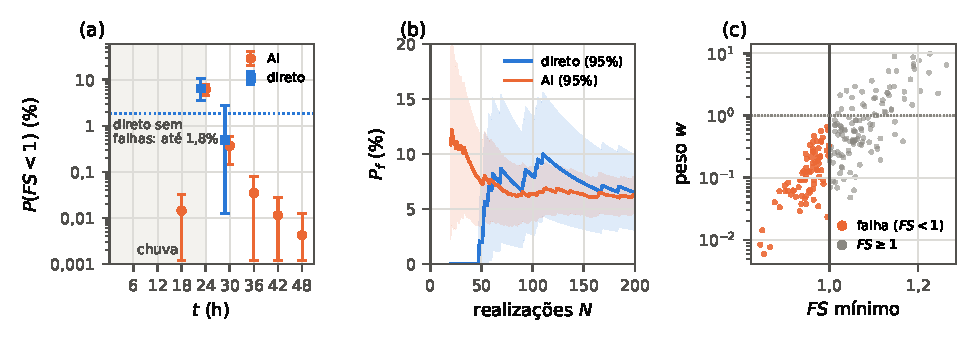
\includegraphics[width=\linewidth]{fig_e0_chuva.pdf}
\caption{Chuva: (a) $P(FS < 1)$ em cada instante, na AI (barras: $P_f(1 \pm 1{,}96\,CoV)$, cortadas no fundo do eixo
quando a ponta de baixo é negativa) e no direto onde ele tem falhas (IC exato), com o limite de 95\% do direto sem
falhas; (b) $P_f$ com o número de realizações e a faixa de 95\%; (c) peso de cada realização da AI contra o $FS$
mínimo.}\label{fig:chuva}
\end{figure}

\paragraph{A $P_f$ em cada instante.} O peso não depende do instante, então a mesma amostra dá a $P_f$ de cada um
(Tab.~\ref{tab:instantes}, Fig.~\ref{fig:chuva}a). A $P_f$ do mínimo é a de \ChDetT~h: o mínimo cai em \ChDetT~h em
\ChMinNoDet{} das \ChNP{} realizações do piloto, e \ChFalhaForaFrase{} noutro instante sem falhar em \ChDetT~h. A AI vê
o que o direto não vê: $P_f = \ChPfADezoito\%$ em \ChTDezoito~h, \ChPfATrinta\% em \ChTTrinta~h e \ChPfATrintaSeis\% em
\ChTTrintaSeis~h, com CoV de \ChCovADezoito\%, \ChCovATrinta\% e \ChCovATrintaSeis\%. O direto tem \ChFalhasPTrinta{} em
\ChTTrinta~h e \ChFalhasPDezoito{} em \ChTDezoito{} e \ChTTrintaSeis~h, onde só diz que a $P_f$ fica abaixo de
\ChZeroHi\%. Em \ChZerosA~h, nenhuma realização da AI falha.

\begin{table}[htbp]\centering\footnotesize
\caption{Chuva, instante a instante: o $FS$ do determinístico, a média e o CoV do $FS$ e as falhas no piloto, e a
$P_f$ do piloto e da AI.}\label{tab:instantes}
\begin{tabular}{rrrrrrrr}\toprule
& & \multicolumn{4}{c}{piloto (direto)} & \multicolumn{2}{c}{AI} \\\cmidrule(lr){3-6}\cmidrule(lr){7-8}
$t$ (h) & $FS_{det}$ & $\overline{FS}$ & $CoV(FS)$ (\%) & falhas & $P_f$ (\%) & $P_f$ (\%) & $CoV$ (\%) \\\midrule
\ChLinhasInstantes
\bottomrule\end{tabular}\end{table}

\subsection{Ganho e teoria}
Num estado limite linear com $P_f = \ChAPf\%$ ($\beta = \ChBeta$), o deslocamento ótimo da entropia cruzada tem
$m^2 = \ChMdois$, e o ganho seria \ChGanhoLinear{} (Seção~7 do \texttt{relatorio\_chuva.pdf}: $m = \varphi(\beta)/P_f$
e segundo momento $e^{m^2}\Phi(-\beta - m)$). Com o $|\mu|^2 = \ChMuDois$ usado, na direção exata, ainda seria
\ChGanhoLinearMu: o tamanho do deslocamento quase não importa. A AI mediu \ChGanho, \ChFracGanho\% do ótimo
(Fig.~\ref{fig:amostra}c). A perda vem da direção: a banda do determinístico aproxima o mecanismo, e o $FS$ não é
linear nos $\xi$. No rebaixamento, a mesma AI fez \RbFracGanhoBanda\% do ótimo (\RbGanhoBanda{} de \RbGanhoLinear).

\subsection{Por que a \texorpdfstring{$P_f$}{Pf} é de uns \ChAPfArred\% e não de \ChPfEsperada\%}
O \texttt{relatorio\_chuva.pdf} esperava $P_f \approx \ChPfEsperada\%$ pelo piloto antigo, de \ChVelhoN{} realizações e
\ChVelhoNf{} falhas: $\overline{FS} = \ChVelhoMedia$ em \ChDetT~h, $CoV = \ChVelhoCov\%$ e $P_f = \ChVelhoLogn\%$ no ajuste
log-normal. Essas \ChVelhoN{} são as realizações \ChVelhoPrimeira{} a \ChVelhoUltima{} daqui (a mesma semente e o mesmo
caso), e o $FS(\ChDetT\text{ h})$ delas muda no máximo \ChVelhoDifMax. O que mudou foi o tamanho da amostra
(Fig.~\ref{fig:amostra}b):
\begin{itemize}
\item as \ChNP{} espalham mais: $CoV = \ChDuzCov\%$, contra \ChOitoCov\% nas \ChVelhoN{} primeiras; a média muda pouco
(\ChDuzMedia{} contra \ChOitoMedia). O ajuste log-normal das \ChNP{} dá \ChDuzLogn\%, perto dos \ChPPf\% contados;
\item o espalhamento pesa mais que a média: com a média das \ChNP{} e o espalhamento das \ChVelhoN, a log-normal daria
\ChCruzA\%; com a média das \ChVelhoN{} e o espalhamento das \ChNP, \ChCruzB\%;
\item com \ChVelhoNf{} falhas em \ChVelhoN, o intervalo exato de 95\% ia até \ChVelhoHi\%: o piloto antigo não separava
\ChPfEsperada\% de \ChAPfArred\%.
\end{itemize}
Com uns \ChAPfArred\%, o direto já vê falhas: para $CoV(P_f) = \ChCovAlvo\%$, ele pede umas \ChNAlvoCov{} realizações,
\ChCpuAlvo~h de CPU no fermi (\ChRelogioAlvo~h com \ChProcessos{} processos).

\begin{figure}[htbp]\centering
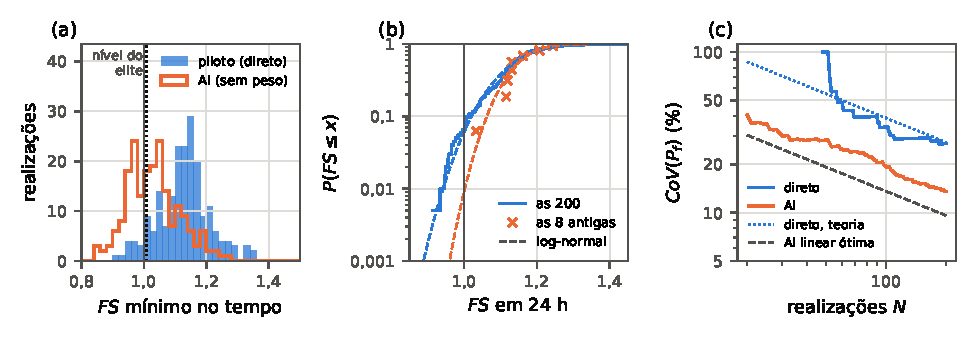
\includegraphics[width=\linewidth]{fig_e0_amostra.pdf}
\caption{Chuva: (a) $FS$ mínimo no piloto e na AI (sem peso), com o nível do conjunto elite; (b) distribuição do
$FS$ em \ChDetT~h nas \ChNP{} realizações do piloto e nas \ChVelhoN{} do piloto antigo, com as log-normais ajustadas;
(c) $CoV(P_f)$ com o número de realizações, com o direto na teoria e a AI ótima de um estado limite linear, as duas
com a $P_f$ da AI.}\label{fig:amostra}
\end{figure}

\section{Cho (2010): a prévia do PC}\label{sec:cho}
\subsection{O problema e as rodadas}
\begin{itemize}
\item \textbf{Problema:} o talude seco do Exemplo~2 de Cho (2010), com $c'$ log-normal de média \ChoC~kPa e
$CoV = \ChoCovC$, $\varphi'$ log-normal de média $\ChoPhi^\circ$ e $CoV = \ChoCovPhi$, e $\gamma = \ChoGamma$~kN/m$^3$.
Aqui o solo é Mohr--Coulomb associado, com $E = \ChoE$~MPa e $\nu = \ChoNu$, e o fator é o do SRM com \texttt{\ChoMalha} e
\ChoNref{} níveis de refinamento.
\item \textbf{Campos:} correlação exponencial com $l_h = \ChoLh$~m e $l_v = \ChoLv$~m e KL com \ChoKLM{} termos por campo
(\ChoKLvar\% da variância). A correlação cruzada $r$ entra nos campos gaussianos: o de $\varphi'$ é
$r\,Z_c + \sqrt{1 - r^2}\,Z_\varphi$, com os mesmos modos, e os $\xi$ continuam independentes.
\item \textbf{Cho:} Bishop com busca da superfície crítica e Monte Carlo com \ChoNmc{} realizações: $FS = \ChoBishop$,
$P_f = \ChoPfCinco\%$ com $r = \ChoRCinco$ (Tabela~5) e $\approx\ChoPfSete\%$ com $r = \ChoRSete$ (Fig.~9).
\item \textbf{Rodadas no PC} (Tab.~\ref{tab:chomc}): o direto com $r = \ChoRCinco$ (alvo de \ChoCincoAlvo; as
\ChoPilotoN{} primeiras são o piloto), a AI dele (\ChoAICincoAlvo), o direto com $r = \ChoRSete$ (\ChoSeteAlvo) e a AI
dele (\ChoAISeteAlvo), na fila do \texttt{cluster/tarefas.sh}, com \ChoProcessos{} processos desde as \ChoInicio{} e
blocos de \ChoBloco; ao lado, os dois FORM. \ifpcparou O PC parou às \PcParou{} (plano, versão 2). A fila faz todos os
blocos do direto antes dos da AI (cada processo só volta aos blocos que esperam o piloto no fim da fila), então as AI não
começaram. O que rodou fica como prévia, com o SRM antigo.\fi
\end{itemize}

\subsection{Determinístico e malha}\label{sec:chomalha}
Com \texttt{tri2} e \ChoNivTriDois{} níveis (\ChoEqTriDois{} equações), o $FS$ é \ChoDetTriDois, a \ChoDifTriDois\% do
Bishop do Cho. Com \ChoNivTriDoisTres{} níveis, ele é \ChoDetTriDoisTres{} (\ChoDifTriDoisTres\%), e com \texttt{tri1}
e \ChoNivTriUm{} níveis (\ChoEqTriUm{} equações), \ChoDetTriUm{} (\ChoDifTriUm\%): o último nível ainda muda o $FS$ em
\ChoUltNivTriDois\% na \texttt{tri2} e \ChoUltNivTriUm\% na \texttt{tri1} (Fig.~\ref{fig:cho}a). Nas realizações, a coluna
\texttt{niveis} dá o mesmo teste: com $r = \ChoRCinco$, o $FS$ do penúltimo nível fica $\ChoCincoNivDif \pm
\ChoCincoNivDp$ acima do último, e as falhas são as mesmas (\ChoCincoNivNf{} contra \ChoCincoNf; \ChoCincoNivTrocas{}
trocas de lado). Com $r = \ChoRSete$, não: \ChoSeteNivNf{} contra \ChoSeteNf{} falhas, \ChoSeteNivTrocas{} troca de
lado. O GIM dá $\Gamma = \ChoDetGim$: num solo $c$--$\varphi$, a
gravidade maior aumenta também a resistência por atrito, e $\Gamma$ é outro fator; a $P_f$ é a mesma, porque $\Gamma < 1$
e $FS < 1$ dizem as duas que o talude não se sustenta. No centro do FORM ($\xi = 0$: as medianas, $c' = \FormCentroC$~kPa
e $\varphi' = \FormCentroPhi^\circ$), $FS = \FormCentroFS$, abaixo do determinístico com as médias.

\subsection{Monte Carlo direto}\label{sec:chodir}
\ifchocincopronto As \ChoCincoN{} realizações com $r = \ChoRCinco$\else\ifpcparou O PC fez \ChoCincoN{} das
\ChoCincoAlvo{} realizações com $r = \ChoRCinco$. Elas\else Até \ChoHoraDados, \ChoCincoN{} das \ChoCincoAlvo{}
realizações com $r = \ChoRCinco$ estavam prontas. Elas\fi\fi{} dão (Tab.~\ref{tab:chomc}, Fig.~\ref{fig:cho}):
\begin{itemize}
\item $P_f = \ChoCincoPf\%$, com \ChoCincoFalhas{} e intervalo \ChoCincoIC{} de \ChoCincoLo\% a \ChoCincoHi\%: os
\ChoPfCinco\% do Cho ficam \ChoCincoDentro{} dele. O $\overline{FS}$ é \ChoCincoMedia, com $CoV(FS) = \ChoCincoCovFS\%$, e
o ajuste log-normal dá \ChoCincoLogn\%;
\item com $r = \ChoRSete$, $P_f = \ChoSetePf\%$ (\ChoSeteFalhas{} em \ChoSeteN; intervalo \ChoSeteIC{} de \ChoSeteLo\% a
\ChoSeteHi\%), com o $\approx\ChoPfSete\%$ do Cho \ChoSeteDentro{} do intervalo. O $CoV(FS)$ é \ChoSeteCovFS\%: com $r$
mais negativo, $c'$ e $\varphi'$ baixos juntos ficam mais raros;
\ifchocincopronto\else
\item \ifpcparou as \ChoCincoEmCurso{} realizações com $r = \ChoRCinco$ em curso quando o PC parou se perderam
(e \ChoSeteEmCurso{} com $r = \ChoRSete$)\else os números parciais tendem um pouco para baixo\fi: uma falha leva
\ChoCustoFalha~s, contra \ChoCustoOutras~s das outras (\ChoCustoRazao{} vezes), então uma realização em curso tem mais
chance de ser falha: \ChoCincoFracCurso\% com $r = \ChoRCinco$, contra \ChoCincoPf\% na amostra. O efeito esperado é de
\ChoCincoFalhasCurso{} falha, menos de meia;
\fi
\item a concordância com o Cho é boa, mas mistura o modelo (elementos finitos contra Bishop), a malha e o viés do SRM
antigo; o plano usa o valor publicado só como plausibilidade.
\end{itemize}

\begin{table}[htbp]\centering\footnotesize\setlength{\tabcolsep}{4.5pt}
\caption{Cho (2010) no PC, SRM antigo: realizações, falhas sorteadas, $P_f$ com o IC de 95\% (exato no direto,
$P_f(1 \pm 1{,}96\,CoV)$ na AI), $CoV = s_q/(\sqrt N P_f)$ e a $P_f$ do Cho.}\label{tab:chomc}
\begin{tabular}{llrrrrrr}\toprule
caso & método & $N$ & falhas & $P_f$ (\%) & IC (\%) & $CoV$ (\%) & Cho (\%) \\\midrule
\ChoLinhas
\bottomrule\end{tabular}\end{table}

\begin{figure}[htbp]\centering
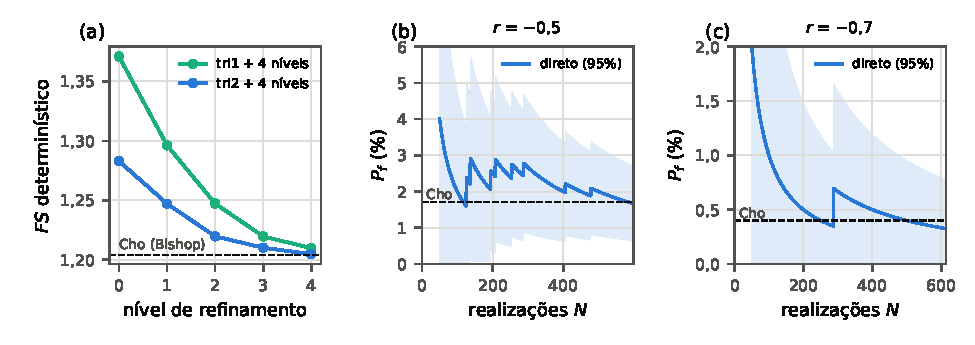
\includegraphics[width=\linewidth]{fig_e0_cho.pdf}
\caption{Cho (2010): (a) $FS$ determinístico por nível de refinamento, com o Bishop do Cho; (b, c) $P_f$ do direto com
o número de realizações e a faixa de 95\%, com a $P_f$ do Cho.}\label{fig:cho}
\end{figure}

\subsection{AI na banda}\label{sec:choai}
\ifchoaicincoiniciado
\ifchoaicincopronto As \ChoAICincoN{} realizações da AI com $r = \ChoRCinco$\else As \ChoAICincoN{} realizações da AI com
$r = \ChoRCinco$ feitas até agora (de \ChoAICincoAlvo)\fi{} \ifchoaicincofalhas dão $P_f = \ChoAICincoPf\%$ com
$CoV = \ChoAICincoCov\%$: \ChoAICincoDif{} desvio do direto, com ganho de \ChoAICincoGanho{} (o ótimo linear é
\ChoGanhoLinCinco)\else ainda não sortearam falha\fi. O conjunto elite são as \ChoAICincoElite{} de menor $FS$, até
$FS < \ChoAICincoNivel$; $s = (\ChoAICincoS)$ para $c'$ e $\varphi'$ e $|\mu|^2 = \ChoAICincoMuDois$. A AI sorteou
\ChoAICincoFalhas, com peso médio \ChoAICincoPeso{} e ESS de \ChoAICincoEss.
\ifchoaiseteiniciado\ifchoaisetefalhas Com $r = \ChoRSete$, a AI dá $P_f = \ChoAISetePf\%$ ($CoV = \ChoAISeteCov\%$,
\ChoAISeteN{} realizações), \ChoAISeteDif{} desvio do direto, com ganho de \ChoAISeteGanho{} (o ótimo linear é
\ChoGanhoLinSete).\else Com $r = \ChoRSete$, a AI ainda não sorteou falha.\fi\fi
\else\ifpcparou
A AI \naoRodou. Com o piloto de \ChoPilotoN{} realizações e uns \ChoCincoPf\% de falhas, o conjunto elite serão as
\ChoEliteN{} de menor $FS$ (menos falhas que \ChoEliteFrac\% do piloto), como na chuva.
\else
Pendente: a fila faz antes todo o direto. Com \ChoCustoMedio~s por realização, a AI começa por volta das \ChoInicioAI,
o direto acaba por volta das \ChoFimDireto, e a campanha não acaba antes das \ChoFimMin.
\fi\fi

\subsection{FORM com \texorpdfstring{$M$}{M} termos por campo}
O \texttt{form\_kl.py} faz o FORM (HL-RF) com $g = FS - 1$ e $r = \ChoRCinco$ nos $2M$ primeiros $\xi$ da KL dos dois
campos, com os outros em zero. $M = \FormDezM$ retém \FormDezVar\% da variância, e $M = \FormVinteM$, \FormVinteVar\%
(contra \ChoKLvar\% no Monte Carlo). O gradiente é por diferenças centrais com passo $h = \FormH$ em $u$: $4M + 1$
avaliações do $FS$ por iteração (\FormDezAvalIt{} e \FormVinteAvalIt). O \texttt{form\_kl.py} para com $|g| < \FormTolG$
e passo menor que \FormTolP; a etapa~2 do plano pede $|g| < \FormTolGNovo$ e $\beta$ mudando menos que \FormTolBNovo{}
(Tab.~\ref{tab:form}, Fig.~\ref{fig:form}).
\begin{itemize}
\item \ifformdezpronto Com $M = \FormDezM$, o FORM \FormDezConvergiu{} (\FormDezAval{} avaliações):
$\beta = \FormDezBeta$ e $P_f = \Phi(-\beta) = \FormDezPf\%$.\else Com $M = \FormDezM$, o FORM \ifpcparou parou com o PC
na\else está na\fi{} iteração \FormDezItAtual{} (\FormDezFeitas{} de \FormDezAvalIt{} avaliações). Na iteração
\FormDezUltIt, $g = \FormDezG$ e $\beta = \FormDezBeta$, ou $P_f = \Phi(-\beta) = \FormDezPf\%$; $\beta$ mudou
\FormDezDBeta{} na última iteração, e o critério da etapa~2 \FormDezCritNovo.\fi{}
\ifformdezpassoacima O critério do \texttt{form\_kl.py} não pararia: o passo em $u$ fica em \FormDezPassoMin{} a
\FormDezPasso{} desde a iteração 3, por ruído do gradiente ($h = \FormH$), acima da tolerância \FormTolP.\fi
\item \ifformvintepronto Com $M = \FormVinteM$, o FORM \FormVinteConvergiu{} (\FormVinteAval{} avaliações):
$\beta = \FormVinteBeta$ e $P_f = \FormVintePf\%$.\else Com $M = \FormVinteM$, o FORM \ifpcparou parou com o PC
na\else está na\fi{} iteração \FormVinteItAtual{} (\FormVinteFeitas{} de \FormVinteAvalIt{} avaliações). Na iteração
\FormVinteUltIt, $g = \FormVinteG$ e $\beta = \FormVinteBeta$ ($P_f = \FormVintePf\%$); $\beta$ mudou \FormVinteDBeta, e o
critério da etapa~2 \FormVinteCritNovo{} (o próximo passo iria a $\beta = \FormVinteBetaProx$).\fi{}
\ifformdezpronto\ifformvintepronto Com mais termos, $\beta$ fica \FormCompara.\fi\fi
\ifpcparou\ifformvintepronto\else Com mais termos, $\beta$ cai de \FormDezBeta{} para \FormVinteBeta, como o plano
espera, mas sem convergência com $M = \FormVinteM$.\fi\fi
\item A $P_f$ do Cho corresponde a $\beta = \ChoBetaCinco$, e a do direto, a $\beta = \ChoBetaDireto$. O FORM vê só
parte da variância e lineariza o $FS$; a AI com o ponto de projeto diz quanto isso pesa.
\item \textbf{Importâncias.} Os maiores $\alpha^2$ com $M = \FormDezM$ são \FormDezTop; por campo, o $\varphi'$ leva
\FormDezAlfaPhi{} e o $c'$, \FormDezAlfaC{} (com $M = \FormVinteM$: \FormVinteAlfaPhi{} e \FormVinteAlfaC). O $c'$ pesa
pouco por causa da correlação cruzada negativa: o $\xi$ do primeiro termo de $c'$ sobe o $c'$ e, com $r = \ChoRCinco$,
baixa o $\varphi'$. Pela regra da cadeia, o efeito dele no $FS$ é de \FormViaC{} por unidade pelo $c'$ e de
\FormViaPhi{} pelo $\varphi'$: sobra \FormGradC, contra \FormGradPhi{} do primeiro termo de $\varphi'$.
\item \textbf{A AI com o ponto de projeto} \ifaiforminiciado (\AIFormN{} realizações) \ifaiformfalhas dá
$P_f = \AIFormPf\%$ ($CoV = \AIFormCov\%$), \AIFormDif{} desvio do direto, com ganho de \AIFormGanho{} e
$|\mu|^2 = \AIFormMuDois$.\else ainda não sorteou falha.\fi\else\ifpcparou \naoRodou; lá, o FORM roda antes da
fila. \else espera o fim do FORM com $M = \FormDezM$. \fi O deslocamento terá $|\mu|^2 = \beta^2 \approx \AIFormMuDois$, e
a variância dos pesos, $e^{|\mu|^2} - 1 \approx \AIFormVarPeso$, contra \ChVarPeso{} na chuva.\fi
\end{itemize}

\begin{table}[htbp]\centering\footnotesize
\caption{FORM do Cho (2010) com $r = \ChoRCinco$: $g = FS - 1$ no ponto de cada iteração e $\beta = |u|$.}
\label{tab:form}
\begin{tabular}{rrrrr}\toprule
& \multicolumn{2}{c}{$M = \FormDezM$} & \multicolumn{2}{c}{$M = \FormVinteM$} \\\cmidrule(lr){2-3}\cmidrule(lr){4-5}
iteração & $g$ & $\beta$ & $g$ & $\beta$ \\\midrule
\FormLinhas
\bottomrule\end{tabular}\end{table}

\begin{figure}[htbp]\centering
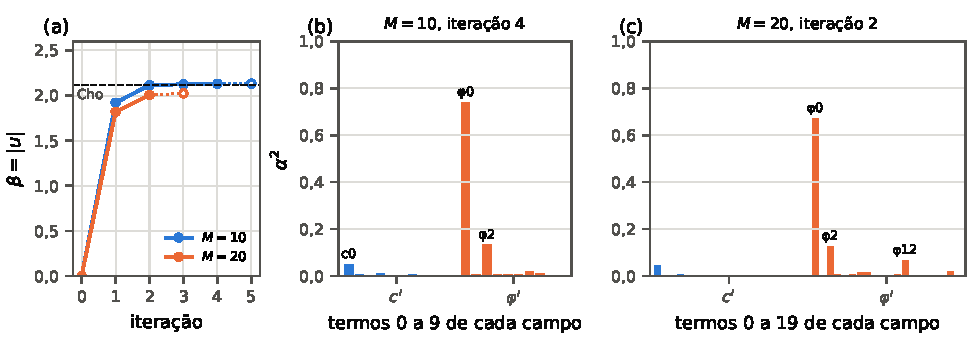
\includegraphics[width=\linewidth]{fig_e0_form.pdf}
\caption{FORM do Cho (2010): (a) $\beta$ por iteração (círculo vazado: o próximo ponto do HL-RF, sem avaliar), com o
$\beta$ da $P_f$ do Cho; (b, c) $\alpha^2$ de cada termo na última iteração, com $M = \FormDezM$ e
$M = \FormVinteM$.}\label{fig:form}
\end{figure}

\section{Balanço das validações da AI até aqui}\label{sec:balanco}
A Tab.~\ref{tab:balanco} junta os casos; o rebaixamento rápido (Seção~6.1 do Ceron, com o transiente) vem do
\texttt{relatorio\_rebaixamento.pdf}.
\begin{itemize}
\item \textbf{Sem sinal de viés, mas o teste é fraco.} Nos \BalNCasos{} casos completos, a maior diferença entre a AI e o
direto é de \BalMaxDif{} desvio (\BalVies). O teste de dois desvios só pega metade das vezes um viés de 1,96 desvio da
diferença: \RbVmdBanda\% da $P_f$ no rebaixamento com a banda e \ChVmd\% na chuva, que tem só \ChNP{} realizações diretas.
\item \textbf{A direção da banda rende \BalFracMin\% a \BalFracMax\% do ótimo linear.} Os primeiros modos rendem bem
menos (\RbGanhoModos{} contra \RbGanhoBanda{} no rebaixamento): o deslocamento de \RbKModos{} modos por campo tem ruído
em direções que não importam.
\item \textbf{O ganho cresce quando a $P_f$ cai:} \RbGanhoBanda{} com $P_f = \RbPfDireto\%$ e \ChGanho{} com \ChAPf\%.
O Cho, com $P_f$ de uns \ChoCincoPf\% e \ChoSetePf\%, tem ótimo linear de \ChoGanhoLinCinco{} e \ChoGanhoLinSete{}
vezes: é onde a AI deve compensar, e é o que falta medir.
\item \textbf{O $k$ aleatório.} No rebaixamento, com $k_v$ fixo, a $P_f$ das mesmas \RbKNPar{} realizações cai de
\RbKPfAleat\% para \RbKPfFixo\% (McNemar $p \RbKMcNemar$): lá o $k$ pesa. Na chuva, o deslocamento quase não mexe no $k$.
\end{itemize}

\begin{table}[htbp]\centering\footnotesize\setlength{\tabcolsep}{4pt}
\caption{As validações da AI: $P_f$ (\%) do direto e da AI, com $N$ ($^\dagger$: parcial); diferença em desvios; viés
mínimo detectável (o que o teste de dois desvios pega metade das vezes, em \% da $P_f$); ganho medido e o ótimo de um
estado limite linear com a mesma $P_f$ (no Cho, a do direto).}\label{tab:balanco}
\begin{tabular}{llrrrrrr}\toprule
caso & deslocamento & direto & AI & diferença & viés mín. & ganho & ótimo \\\midrule
\BalLinhas
\bottomrule\end{tabular}\end{table}

\section{O que passa para a etapa 1}\label{sec:etapa1}
A etapa~1 do plano compara o SRM antigo com o corrigido (o caminho de $F$ começa em $F_0 = \EtapaUmFzero$) nas mesmas
realizações, no fermi: as \EtapaUmPar{} primeiras do Cho com $r = \ChoRCinco$ e \EtapaUmChuva{} da chuva. Ela roda com
os casos do Cho da etapa~0 na campanha \texttt{etapa1} (\texttt{cluster/casos\_etapa1.txt}). A etapa~0 deixa para ela:
\begin{enumerate}
\item \textbf{A conferência entre máquinas.} As \ChoAntesN{} realizações do PC com $r = \ChoRCinco$ (SRM antigo) estão
entre as \EtapaUmPar{} do \texttt{r05\_antigo}: o $FS$ tem de ser o mesmo. Nelas há \ChoAntesNf{} falhas e
\ChoAntesPerto{} realizações com $FS$ em \ChoAntesFaixa, as candidatas a mudar de lado com o SRM novo.
\item \textbf{A malha e o buraco.} O último nível muda o $FS$ em \ChoCincoNivDif{} (Seção~\ref{sec:chomalha});
com $r = \ChoRCinco$, as falhas são as mesmas, mas, com $r = \ChoRSete$, \ChoSeteNivTrocas{} das \ChoSeteNf{} falhas troca
de lado: com $P_f$ pequena, a malha de teste pode mudar a $P_f$. A malha de teste sai da coluna \texttt{niveis}. A Tab.~\ref{tab:buraco} é a linha de base do
histograma antigo.
\item \textbf{O FORM e a chuva.} O $\beta$ do Cho com o SRM antigo (\FormDezBeta, que \FormDezCritNovo{} no critério da etapa~2, e
\FormVinteBeta\ifformvintepronto\else, ainda sem convergir\fi) é a referência dos FORM da etapa~2. Na chuva, a $P_f$ é de uns \ChAPfArred\%, e o mínimo no tempo cai em \ChDetT~h em \ChMinNoDet{} de \ChNP,
o que apoia o $FS$ em \ChDetT~h da etapa~4.
\end{enumerate}

\appendix
\section{Arquivos lidos e como atualizar}\label{sec:arquivos}
{\raggedright\small
\textbf{Chuva:} \path|~/projects/runs/fermi_chuva_ai| (\path|chuva_ai/ref48_piloto/|, \path|chuva_ai/ref48_ai/|,
\path|chuva_ai/logs/| e \path|resultado.txt|), \path|cluster/casos_chuva_ai.txt| e \path|cluster/README.md|, e o piloto
antigo, no build (\path|mc/gim_I/piloto_srm_I31.05_0_7.csv|). \textbf{Cho:} \path|~/projects/runs/cho2010|
(\path|casos.txt|, \path|rodar.sh|, \path|cadeia_form.sh|, \path|campanha/|, \path|det/|, \path|form_M10_r05/|,
\path|form_M20_r05/| e \path|campanha_form/|) e \path|Projects/Cho2010/| (\path|README.md| e \path|cho2010.cpp|).
\textbf{Contexto:} \path|numeros_rebaixamento.tex|, \path|numeros_solos.tex|, \path|cluster/casos_etapa1.txt| e
\path|PlanoDeTrabalho/README.md|. O script imprime o arquivo de cada número; os resumos pequenos ficam em
\path|ETAPA0/resultados/|. Para atualizar, \texttt{./atualiza.sh} roda o script e compila o relatório numa pasta
temporária; as chaves \texttt{\textbackslash if...pronto}, \texttt{\textbackslash if...iniciado} e \texttt{\textbackslash
ifpcparou} trocam o texto quando uma rodada começa, acaba ou para.\par}

\begin{thebibliography}{9}\small\setlength{\itemsep}{0pt}
\bibitem{cho2010} Cho (2010). Probabilistic assessment of slope stability that considers the spatial variability of
soil properties. \emph{Journal of Geotechnical and Geoenvironmental Engineering} 136(7):975--984.
doi:10.1061/(ASCE)GT.1943-5606.0000309.
\bibitem{rahardjo2007} Rahardjo, Ong, Rezaur e Leong (2007). Factors controlling instability of homogeneous soil slopes
under rainfall. \emph{Journal of Geotechnical and Geoenvironmental Engineering} 133(12):1532--1543.
doi:10.1061/(ASCE)1090-0241(2007)133:12(1532).
\bibitem{rubinstein2004} Rubinstein e Kroese (2004). \emph{The Cross-Entropy Method}. Springer, Nova York.
doi:10.1007/978-1-4757-4321-0.
\bibitem{ceron2025} Vargas Ceron, Cecílio, Linn e Maghous (2025). Stability analysis of slope subjected to seepage forces
considering spatial variability of soil properties. \emph{International Journal for Numerical and Analytical Methods in
Geomechanics} 49(11):2459--2491. doi:10.1002/nag.3993.
\end{thebibliography}
\end{document}
